\chapter{Phase 3: Fein-Design und Installation/Konfiguration}

\section{Package Diagram}
Das Smartwatch besitzt einige interessante Funktionen: einen präzisen Touchscreen, Apps und Widgets, etwa zum Lesen von Mails, SMS, Twitter und Facebook sowie Infos vom gekoppelten Smartphone, etwa über verpasste Anrufe und den Akkustatus.
Standard Anwendungen die mit dem Smartwatch geliefert werden, sind Uhrzeitangaben, Erinnerungsfunktionen, Kalender-Funktionalität, oder die Aktivitätserkennung. 
Klassische Anwendungen sind auch die Fitnessfunktionalitäten.
Mit der mitegelieferten API \textit{AppKit} lassen sich Apps für die SmartWatch programmieren, die eng mit dem Smartpohone zusammenarbeiten.
Die softwaretechnische Paketstruktur ist im Package \textit{Software} abgebildet.

\begin{figure}[h]
\centering\
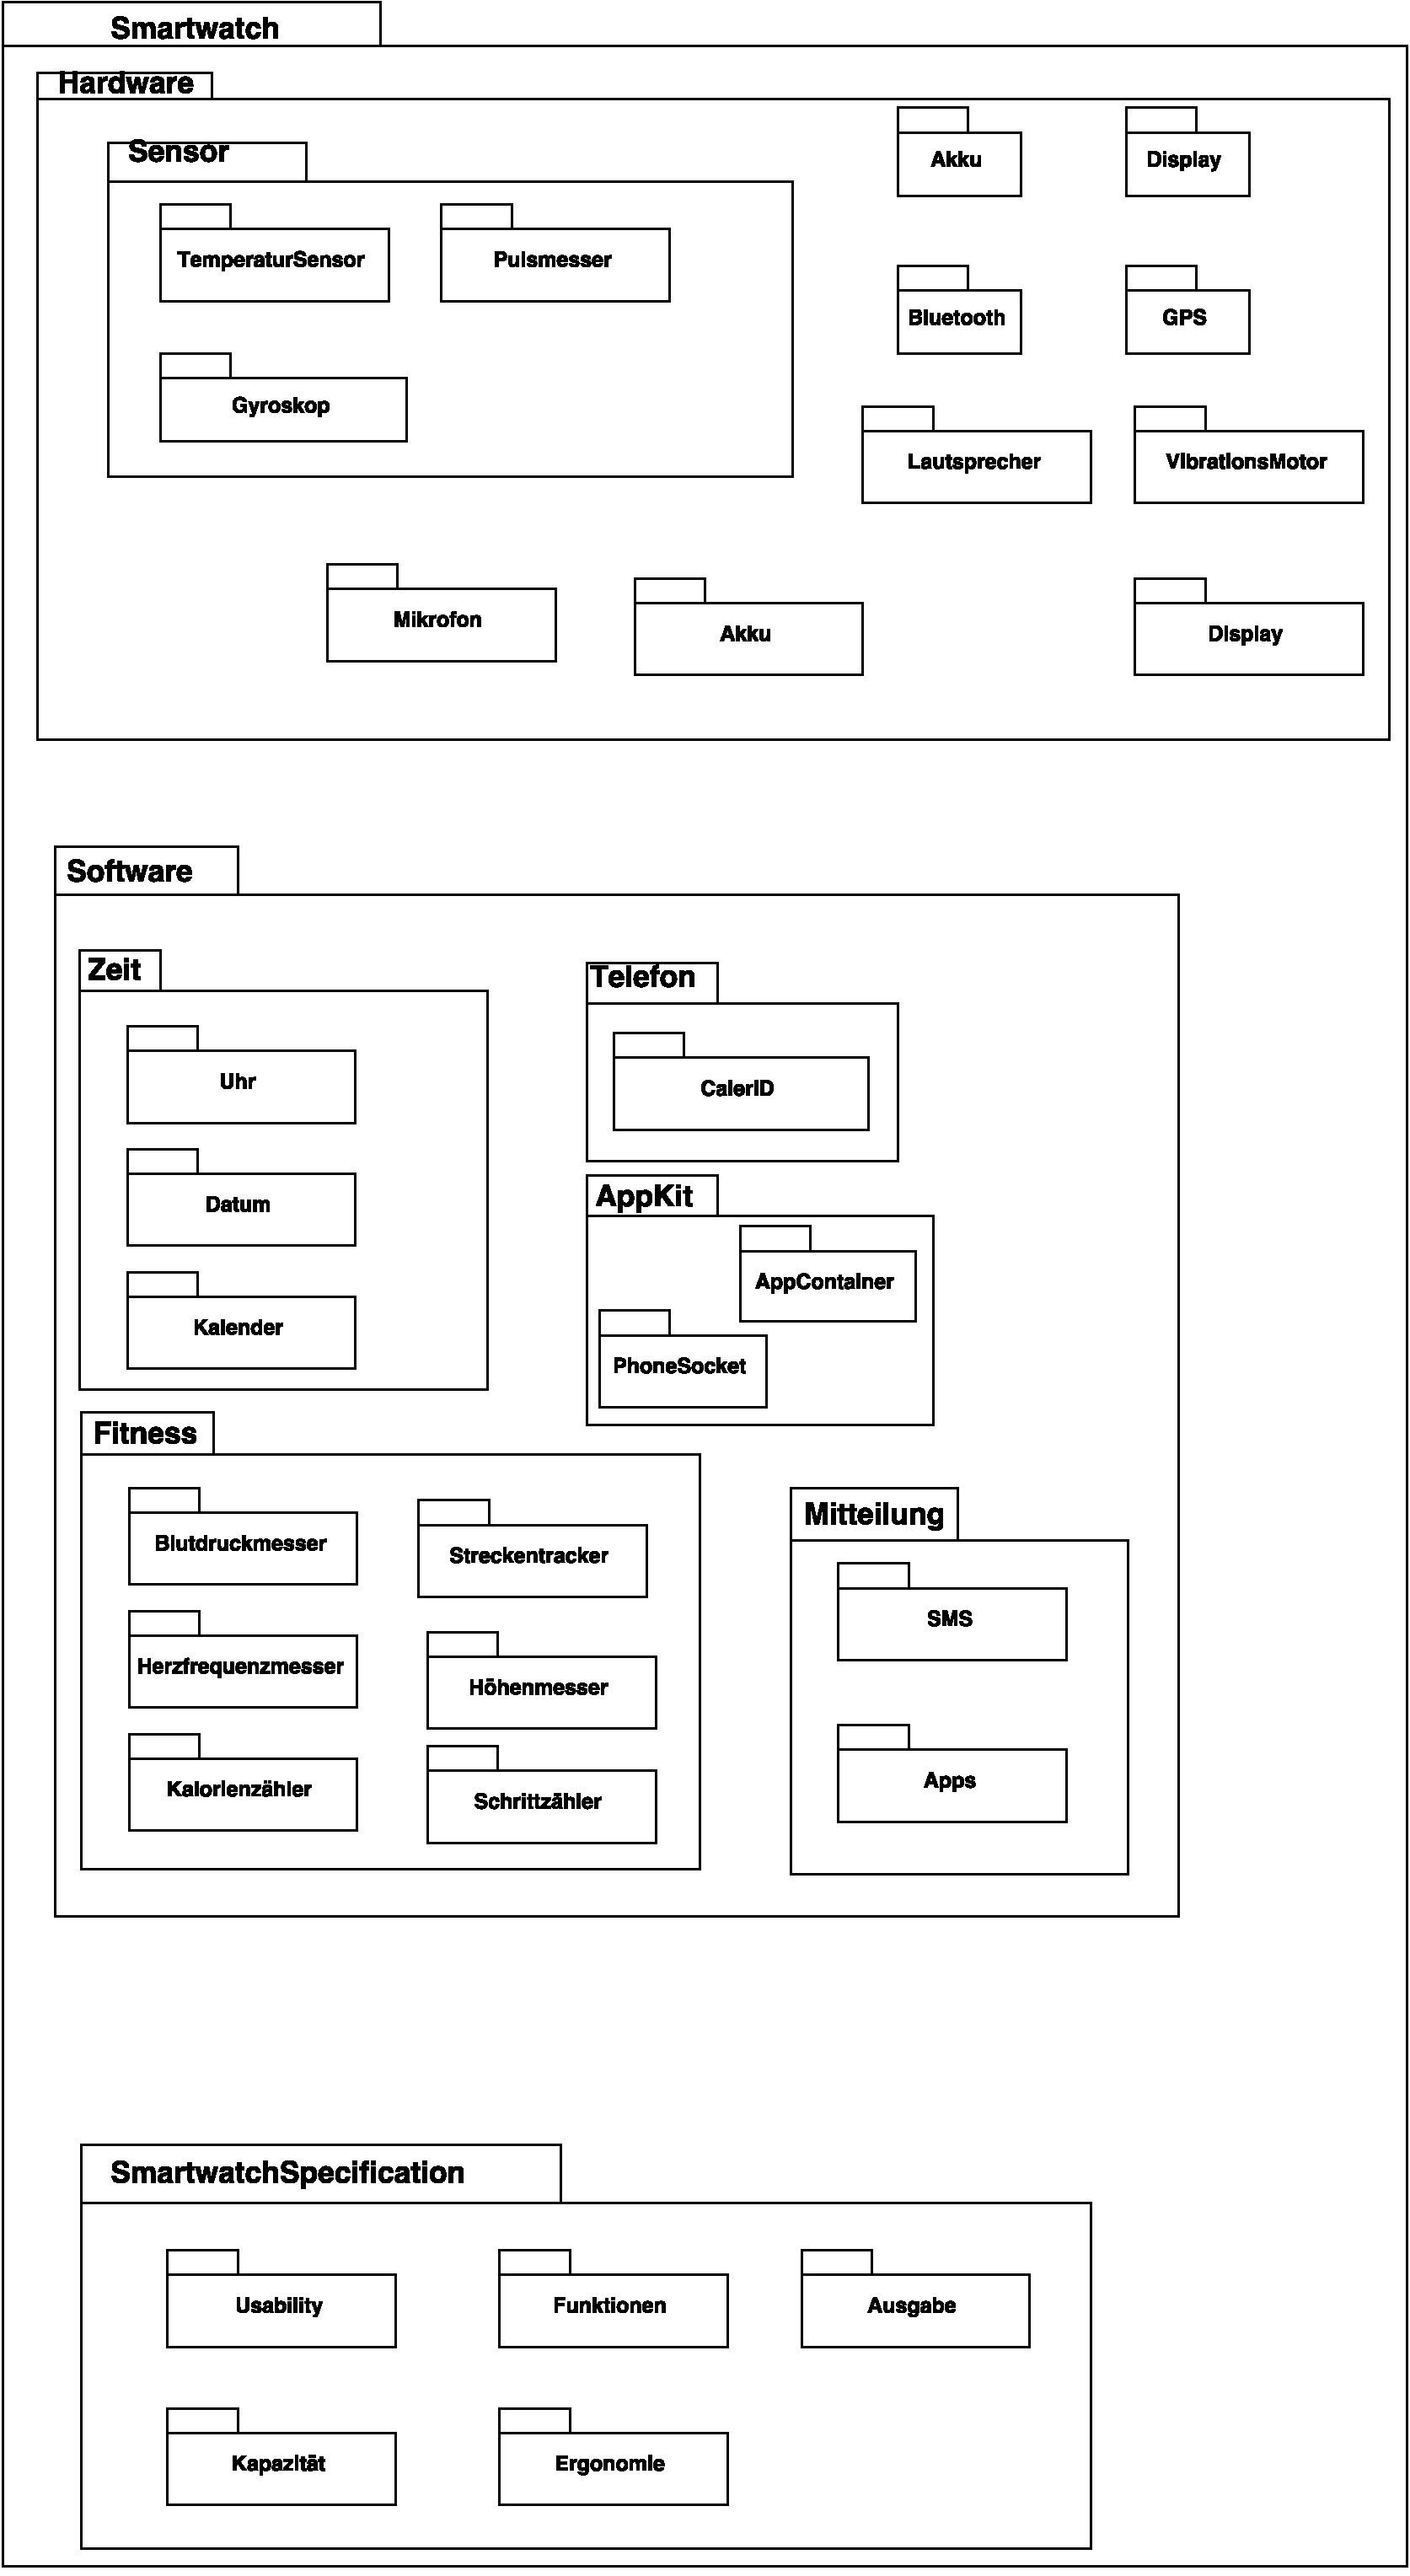
\includegraphics[width=\textwidth]{img/PackagePhase2}
\caption{Packagediagram}\label{fig:package}
\end{figure}

\section{Class Diagram}

Erstmals in \textbf{Phase 3} verwendet, bildet das \textbf{Class Diagram} eine Sammlung von Interfaces und Klassen ab, die in Software realisiert werden sollen. Das Diagramm in Abbildung~\ref{fig:class} beschreibt die drei Hauptmerkmale bzw. Hauptfunktionen der Smartwatch. Das Interface \emph{Zeit} wird den Klassen \emph{Uhr}, \emph{Datum} und \emph{Kalender} implementiert. Instanzen dieser Klassen können sowohl von Systemanwendungen, als auch von Drittanbietern verwendet werden, um beispielsweise eigene Ziffernblätter für die Smartwatch zu entwickeln. Der Entwickler eines Ziffernblatts muss sich dann nicht selbst um den Code zur Zeitmessung oder Kalenderintegration kümmern. Ebenso wird über die Klassen \emph{Herzfrequenzmesser}, \emph{Kalorienzähler}, \emph{Schrittzähler}, \emph{Blutdruckmesser}, \emph{StreckenTracker} und \emph{Höhenmesser}, welche alle das Interface \emph{Fitness} implementieren, ein Framework an Fitness-Trackern bereitgestellt. Drittanbieter-Software kann dieses Framework nutzen, um ein einheitliches Transkript an Fitness-Daten zu verwalten.

Mitteilungen und Benachrichtigungen können von einer App nur dann eingeblendet werden, wenn die App das \emph{Mitteilungen} Interface implementiert. Nicht-Fitness-Anwendungen von Drittanbietern laufen in einer sog. \gls{Sandbox}. Das bedeutet, die Zugriffsrechte der Anwendung sind beschränkt auf den eigenen Datenpool und definierte Schnittstellen. Dieses Regelwerk ist über das Interface \emph{AppKit} definiert, welches von jeder Drittanbietersoftware implementiert werden muss. Die Klassen \emph{PhoneSocket} und \emph{AppContainer} sind Realisierungen dieses Interfaces und erlauben eine Kommunikation der App mit einem Software-Gegenstück auf dem gekoppelten Smartphone bzw. die Zugriffe auf den dedizierten Speicherbereich der App selbst.

\begin{figure}[h]
\centering\
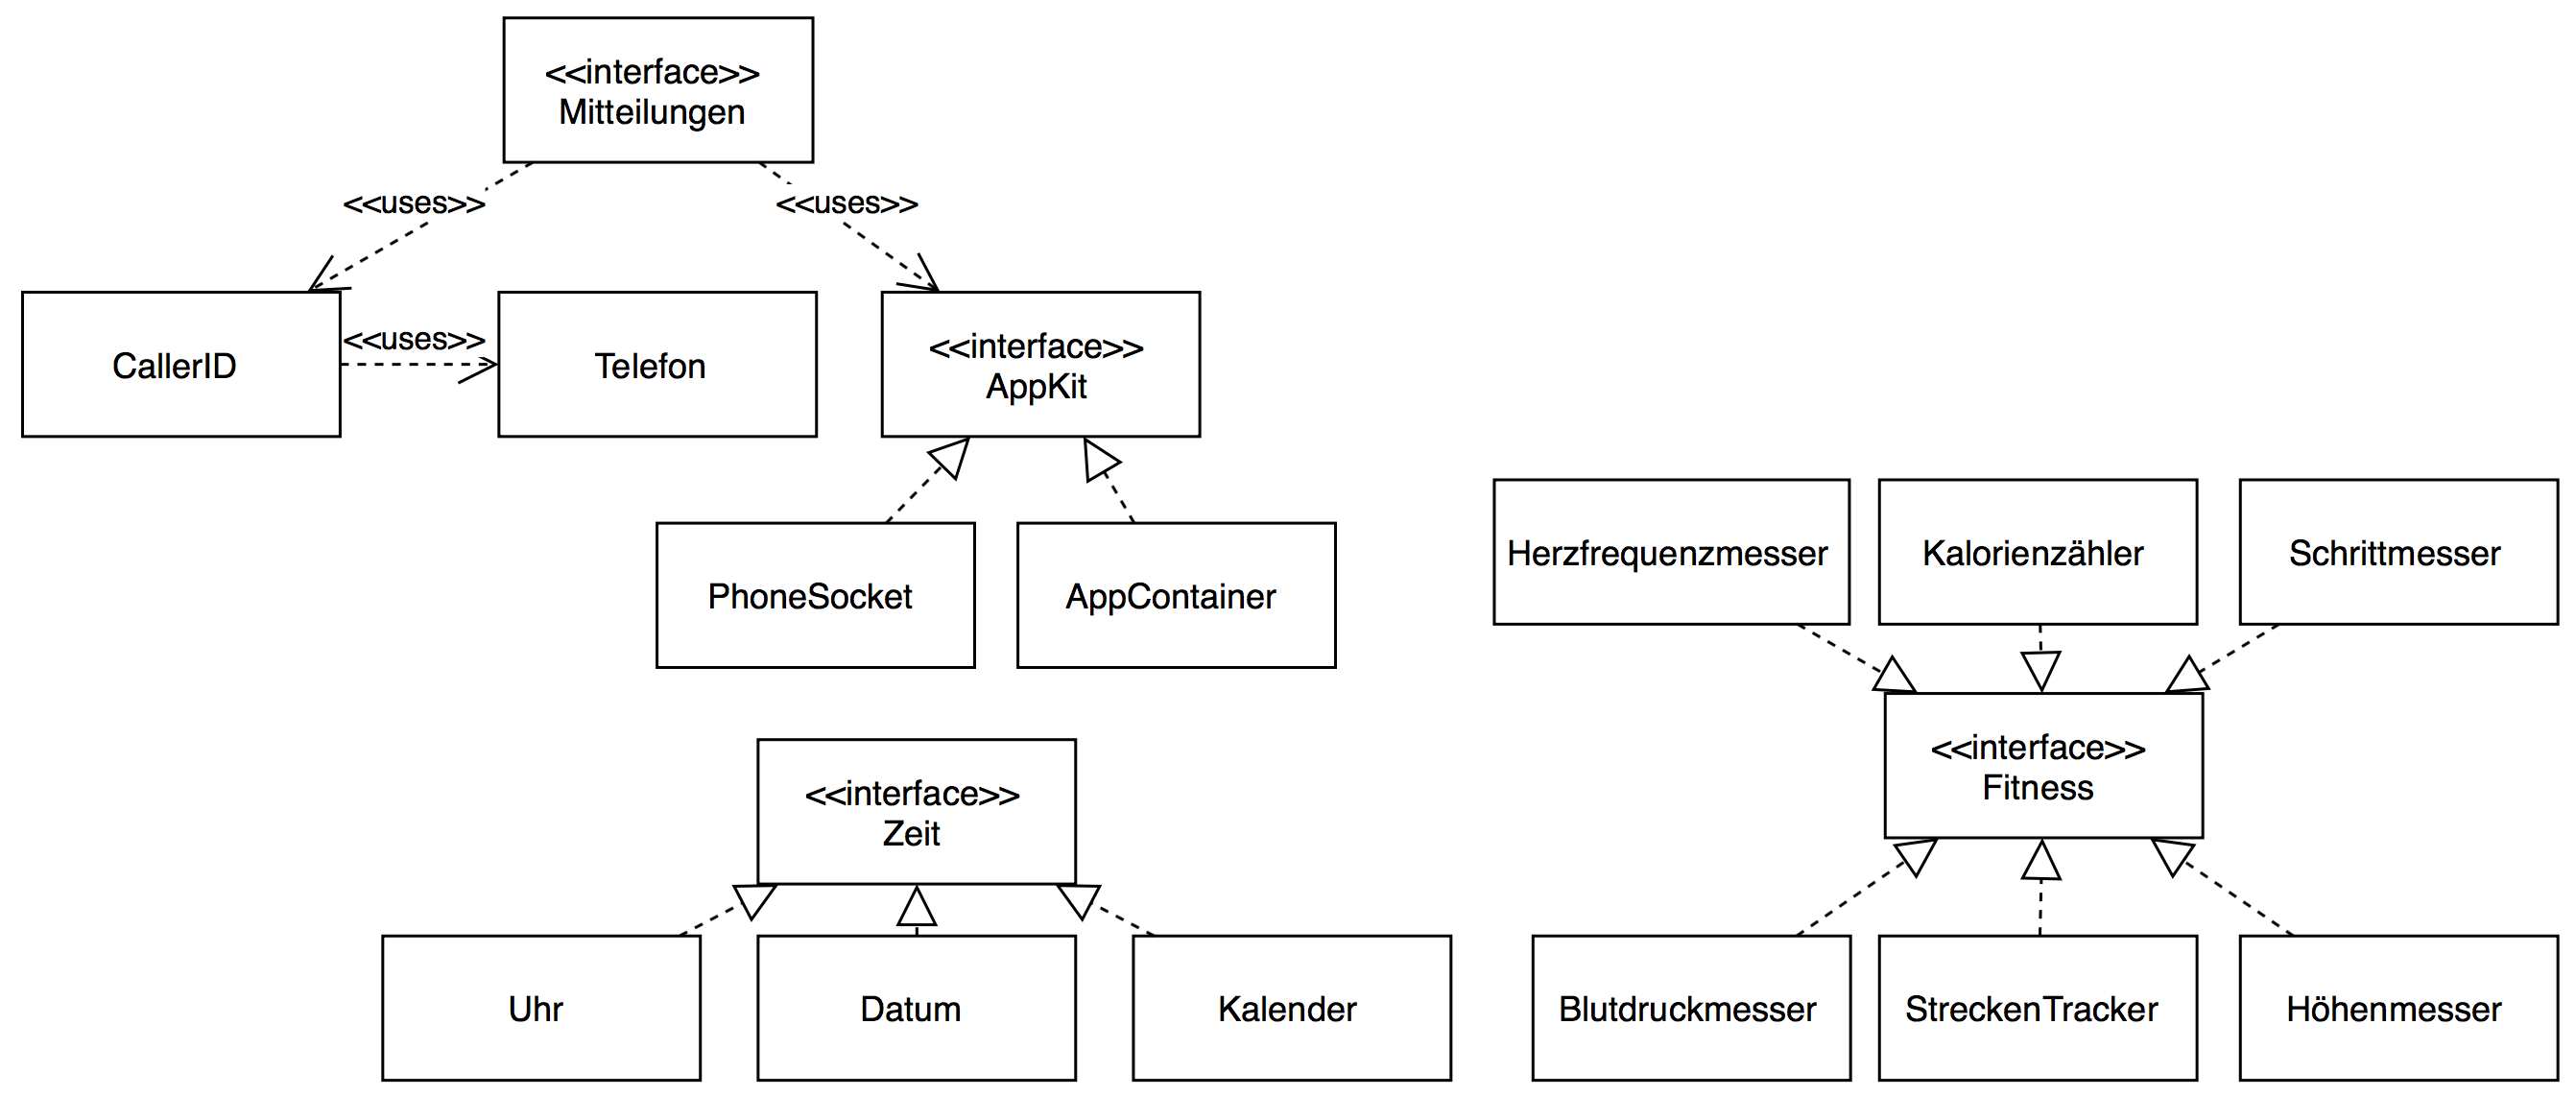
\includegraphics[width=\textwidth]{img/classdiagram}
\caption[Class Diagram: Software-Komponenten]{Relevante Software-Komponenten des Smartwatch-Systems in einem Klassendiagramm}\label{fig:class}
\end{figure}


\section{Block Definition Diagram}
In \textbf{Phase 3} stellt das \textbf{Block Definition Diagram} wieder den \textbf{physikalischen Aufbau} der \textit{SmartWatch} dar \ref{fig:block2}. Da nun alle \textbf{Funktionalitäten} fertig definiert wurden, ist dies der \textbf{endgültige Aufbau} der Uhr. Die zwei \textbf{Hauptkomponenten} der \textit{SmartWatch} sind weiterhin das \textit{SmartWatch-Modul} und das \textit{Armband}. Wobei das \textit{Modul} die \textbf{Funktionalitäten} und die \textbf{Software} verwaltet und das \textit{Armband} die Uhr mit Strom versorgt. Im Zentrum des Diagramms das \textit{SmartWatch-Modul}. Dieses besitzt eine \textit{Bluetooth-Antenne}. Über diese \textbf{Schnittstelle} kommuniziert die \textit{Uhr} mit einem gekoppelten \textit{SmartPhone}. Das \textit{Modul} besitzt einen \textit{Display} dessen Auflösung in Pixel angegeben wird. Dieser wird über \textit{drei} \textit{Tasten} bedient. \textit{Eine Taste} ist das \textit{Zoomrad}. Damit wird die \textbf{Schriftgröße} angezeigter Nachrichten oder laufender Applikationen gesteuert. Zusätzlich kann mit den \textit{Scrolltasten} die \textit{SmartWatch} aus dem \textbf{Ruhezustand} geholt oder nach dem \textbf{Herunterfahren} wieder gestartet werden. Eine weitere Komponente ist der interne \textit{Speicher} zum verwalten der \textbf{nativen Fitnessapplikationen} und \textbf{Fehlerprotokollen}. Außerdem hält das \textit{SmartWatch-Modul} einen \textit{Vibrationsmotor}. Auf diesen \textit{Motor} können \textbf{Applikationen} vom \textit{Smartphone} oder auch die \textbf{nativen Fitnessfunktionen} zugreifen, um den Benutzer über spezielle Ereignisse zu informieren. Für die \textbf{Tonausgabe} bei Verwendung einer \textbf{Musikapplikation} oder bei einem \textbf{Telefonat} ist ein \textit{Lautsprecher} vorhanden. Dieser gibt jede Form von Audiosignal, die sonst über die \textit{SmartPhone-Lautsprecher} ausgegeben werden würde, stattdessen über die \textit{SmartWatch} aus. Das integrierte \textit{Mikrophon} dient als \textbf{Kommunikationsschnittstelle} für Telefonate. Das aufgefangene \textbf{Audiosignal} wird an das \textit{Smartphone} weitergeleitet und dient als Ersatz für das \textit{Mikrophon} im \textit{SmartPhone}. Zur Verwendung durch die \textbf{nativen Fitnessapplikationen} und auch für den Zugriff durch andere \textbf{SmartPhone-Applikationen} stehen ein \textit{GPS-Modul} und \textit{Sensoren} zur Verfügung. Da die \textbf{Fitness-Funktionalität} auch ohne \textit{SmartPhone} ausführbar sein sollen, können dafür nicht die vorhandenen Modalitäten des \textit{SmartPhones} verwendet werden. Als \textit{Sensoren} stellt die \textit{SmartWatch} ein \textit{Gyroskop}, ein \textit{Temperatursensor} und ein \textit{Pulsmesser}. Das \textit{Gyroskop} ermöglicht es, in Verbindung mit dem \textit{GPS}, zurückgelegte Strecken zu messen. Der \textit{Temperatursensor} misst die aktuelle Körpertemperatur über die Haut des Benutzers. Der letzte \textit{Sensor} ist der \textit{Pulsmesser}. Dieser misst den Puls des Benutzer über das Handgelenk.\\
Als nächste \textbf{Hauptkomponente} wird das \textit{Armband} betrachtet. Das \textit{Armband} soll die \textbf{Stromversorgung} der \textit{SmartWatch} regeln und ist austauschbar. So gibt es \textbf{verschiedene Modelle} für \textbf{Fitness} und \textbf{Alltag}. Diese halten eine unterschiedliche Anzahl an \textit{Akkuzellen} und bestehen deshalb aus verschiedenen Materialien. Aus der Verwendung unterschiedlicher Materialien folgt wiederum ein Unterschied in Gewicht und Komfort der \textit{Armbänder}.
\begin{figure}[h]
\centering\
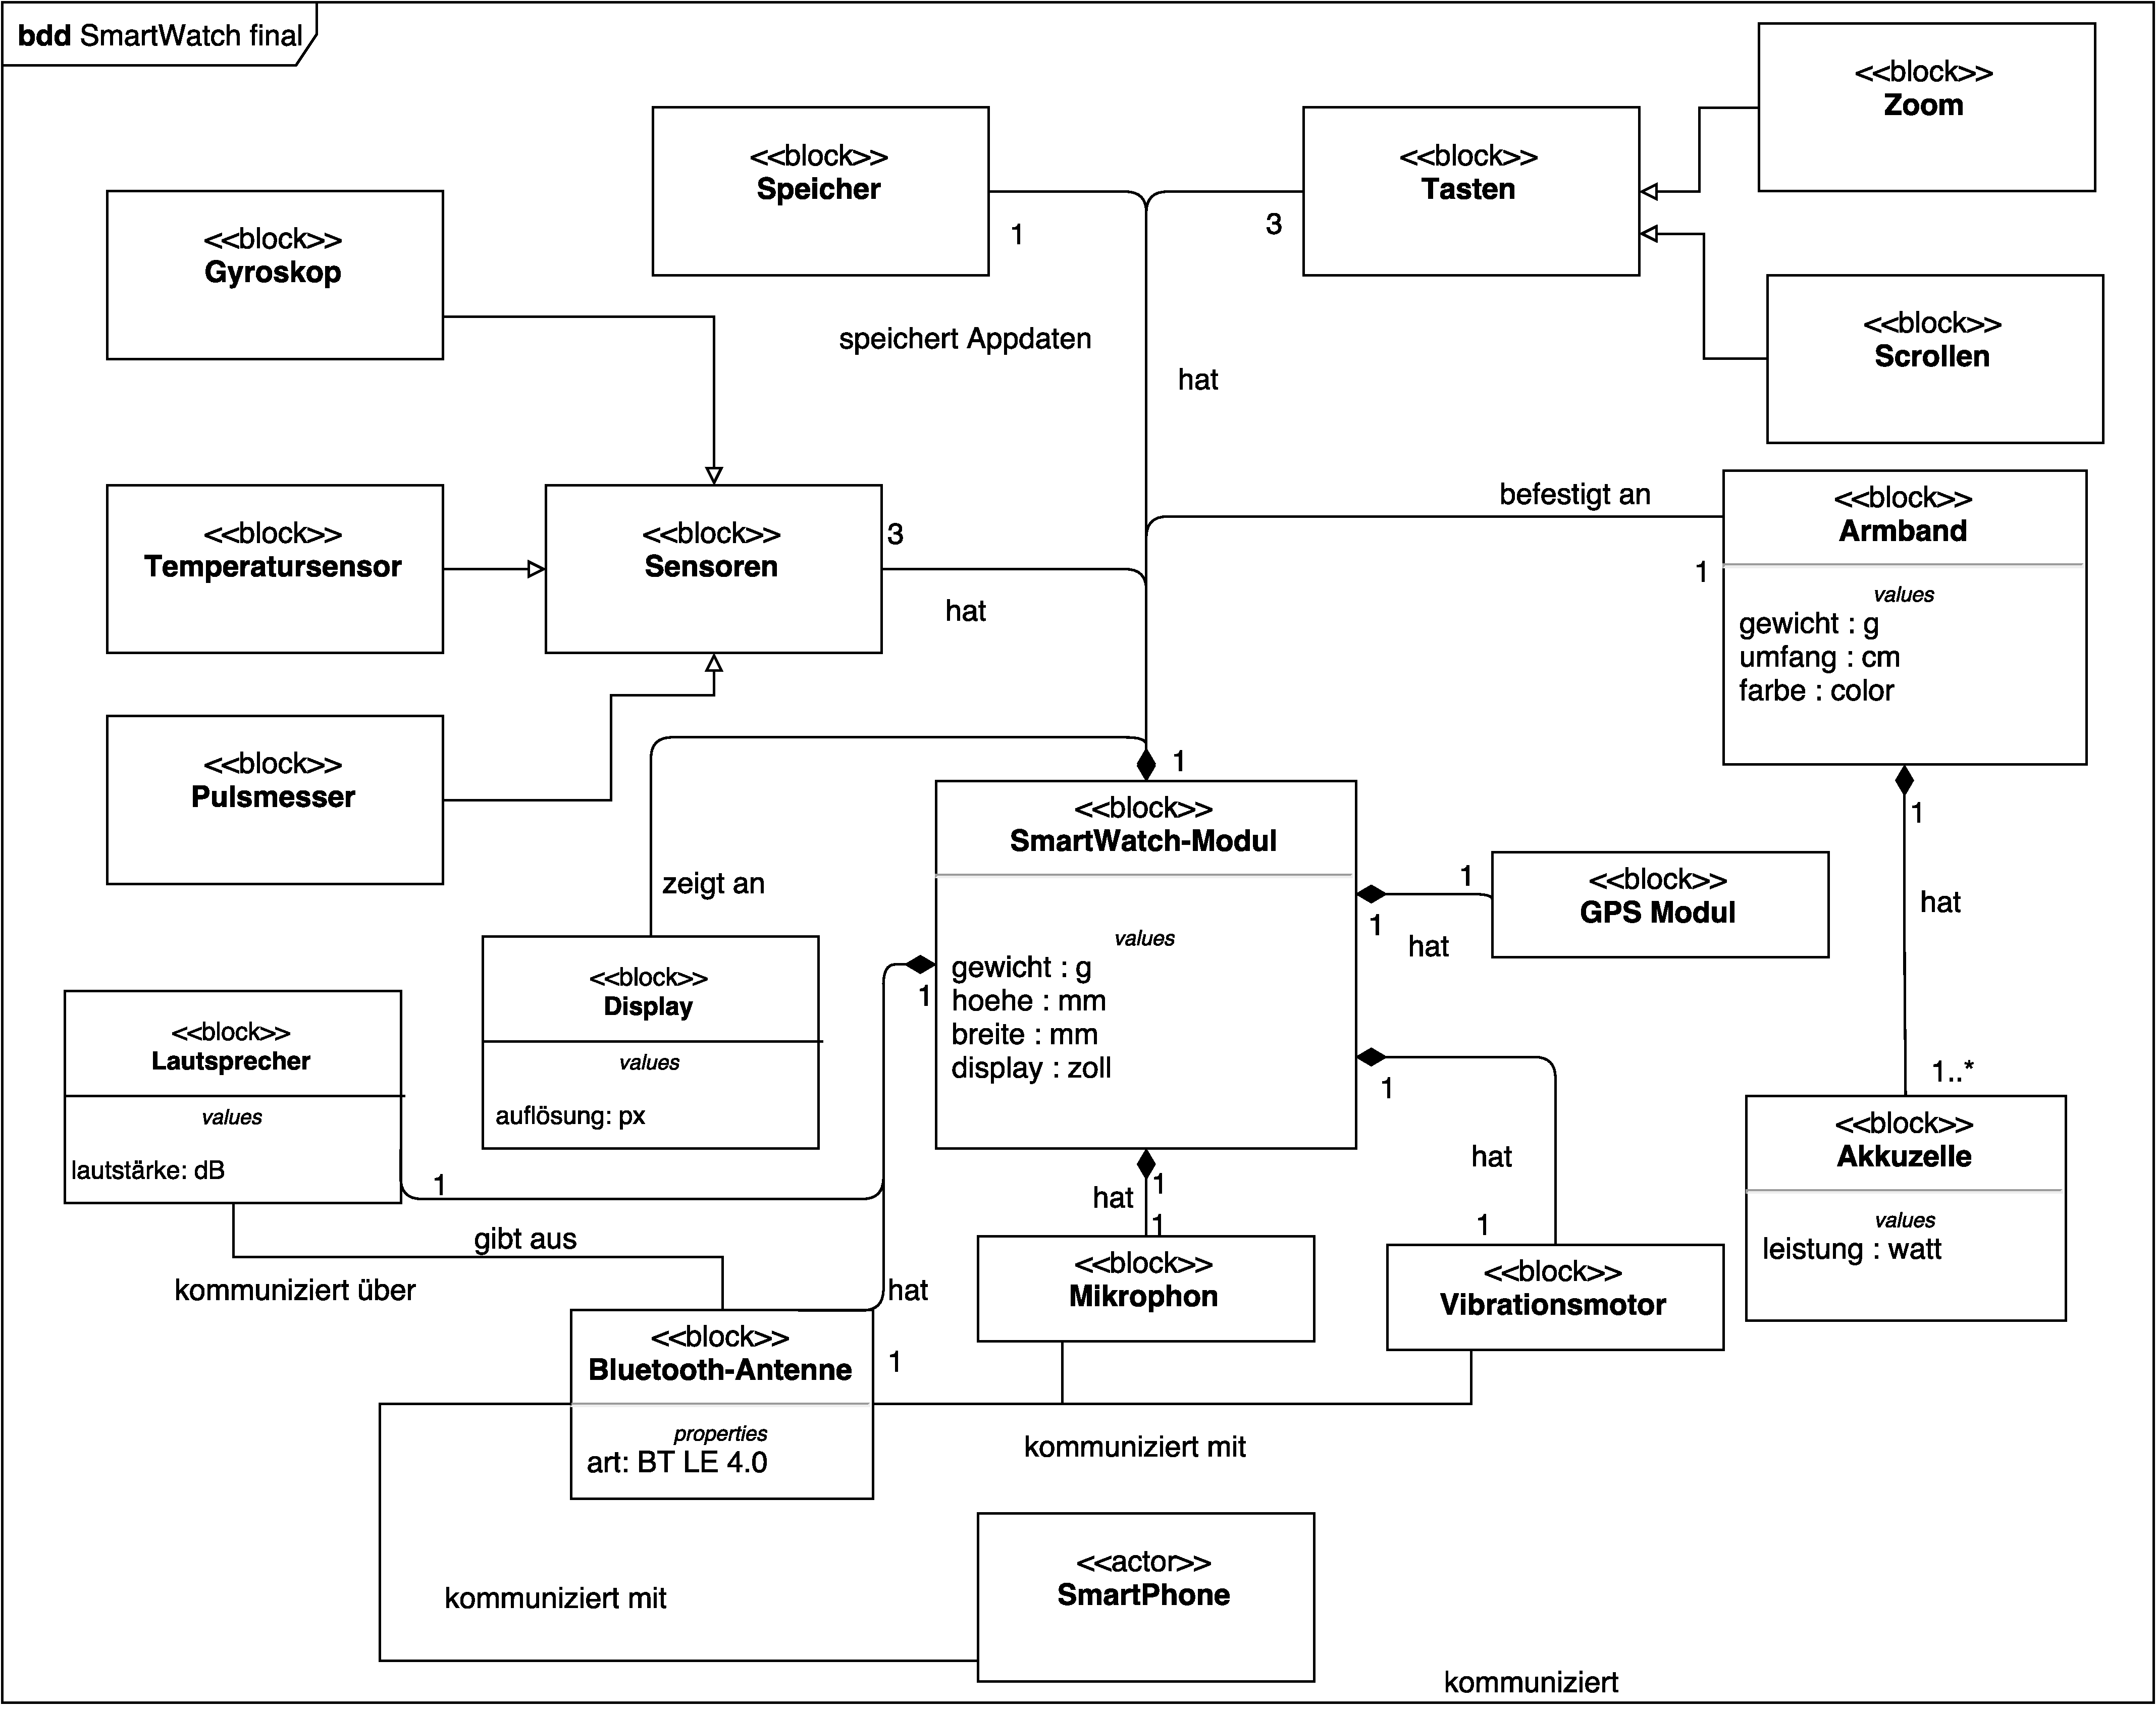
\includegraphics[width=\textwidth]{img/block2}
\caption{Endgültiger physikalischer Aufbau der SmartWatch in Phase 3 anhand eines Block Definition Diagrams.}\label{fig:block2}
\end{figure}

\section{Timing Diagram}

\section{Parametric Diagram}
Im folgenden wird die Anforderung an die Akkulaufzeit ausführlich als Parametric Diagram dargestellt und erläutert.
Da der Verbrauch des Smartwatches von großem Interesse ist, wird der Verbrauch 
mit Analytische Batteriemodelle modelliert.
Außerdem ist in der Anforderung des Smartwatches festgelegt, das die Akkulaufzeit bei normaler Benutzung mindestens 24 Stunden halten muss. %% ref???
Der Verbrauch eines Systems ist die Summe der Verbrauchswerte einzelner Subkomponenten, wie z.B die Sensoren und Benutzersoftware. Die Subkomponenten dienen als Input für die Laufzeitmodellierung des Smartwatches.
Die Constraint Blöcke dienen der graphischen Repräsentation von Bedingungen für die Ladezeit, die für das Smartwatch verwendet werden sollen. 
Analytische Batteriemodelle sind die erste Klasse der Batteriemodelle, welche
hier näher untersucht werden.
Diese beschreiben mathematisch durch eine oder mehrere analytische Gleichungen den Verbrauch einer Batterie zu modellieren.
Eines der ersten und einfachsten analytischen Batteriemodelle ist die Formel
von Peukert, welche die Entladezeit oder auch tatsächlich nutzbare Kapazität
einer Batterie unter einer konstanten Last berechnen kann.\\ %%%%referenz 
Die Formel von Peukert ist wie folgt:
\[
T= \frac{C}{I^{n}}
\]
Die Kapazität \textit{C} ist in Ampere h gegeben.
\textit{I} steht fur den Strom (in Ampere). Der Parameter \textit{n} steht fur die 
Peukert-Zahl von der verwendeten Batterie.\\
Weiterhin gibt es stochastische Batteriemodelle, dass das Entladeverhalten einer Batterie
über einen stochastischen Prozess modeliert.
Das Modell von Panigrahi ist ein stochastisches Modell.
Im Modell wird zwischen der theoretischen Kapazität \textit{T} und der tatsächlich verfugbaren
Kapazität \textit{N} der Batteriezelle unterschieden.
Die Formel ist in der Constraint-Block abgebildet und in der Literatur näher beschrieben.
In der Abbildung \ref{blockBattery} ist ein Block Definition Diagram angefertigt, welche die einzelnen Constraint Blöcke beinhaltet und ihren inneren Aufbau darstellt.

\begin{figure}[H]
\centering\
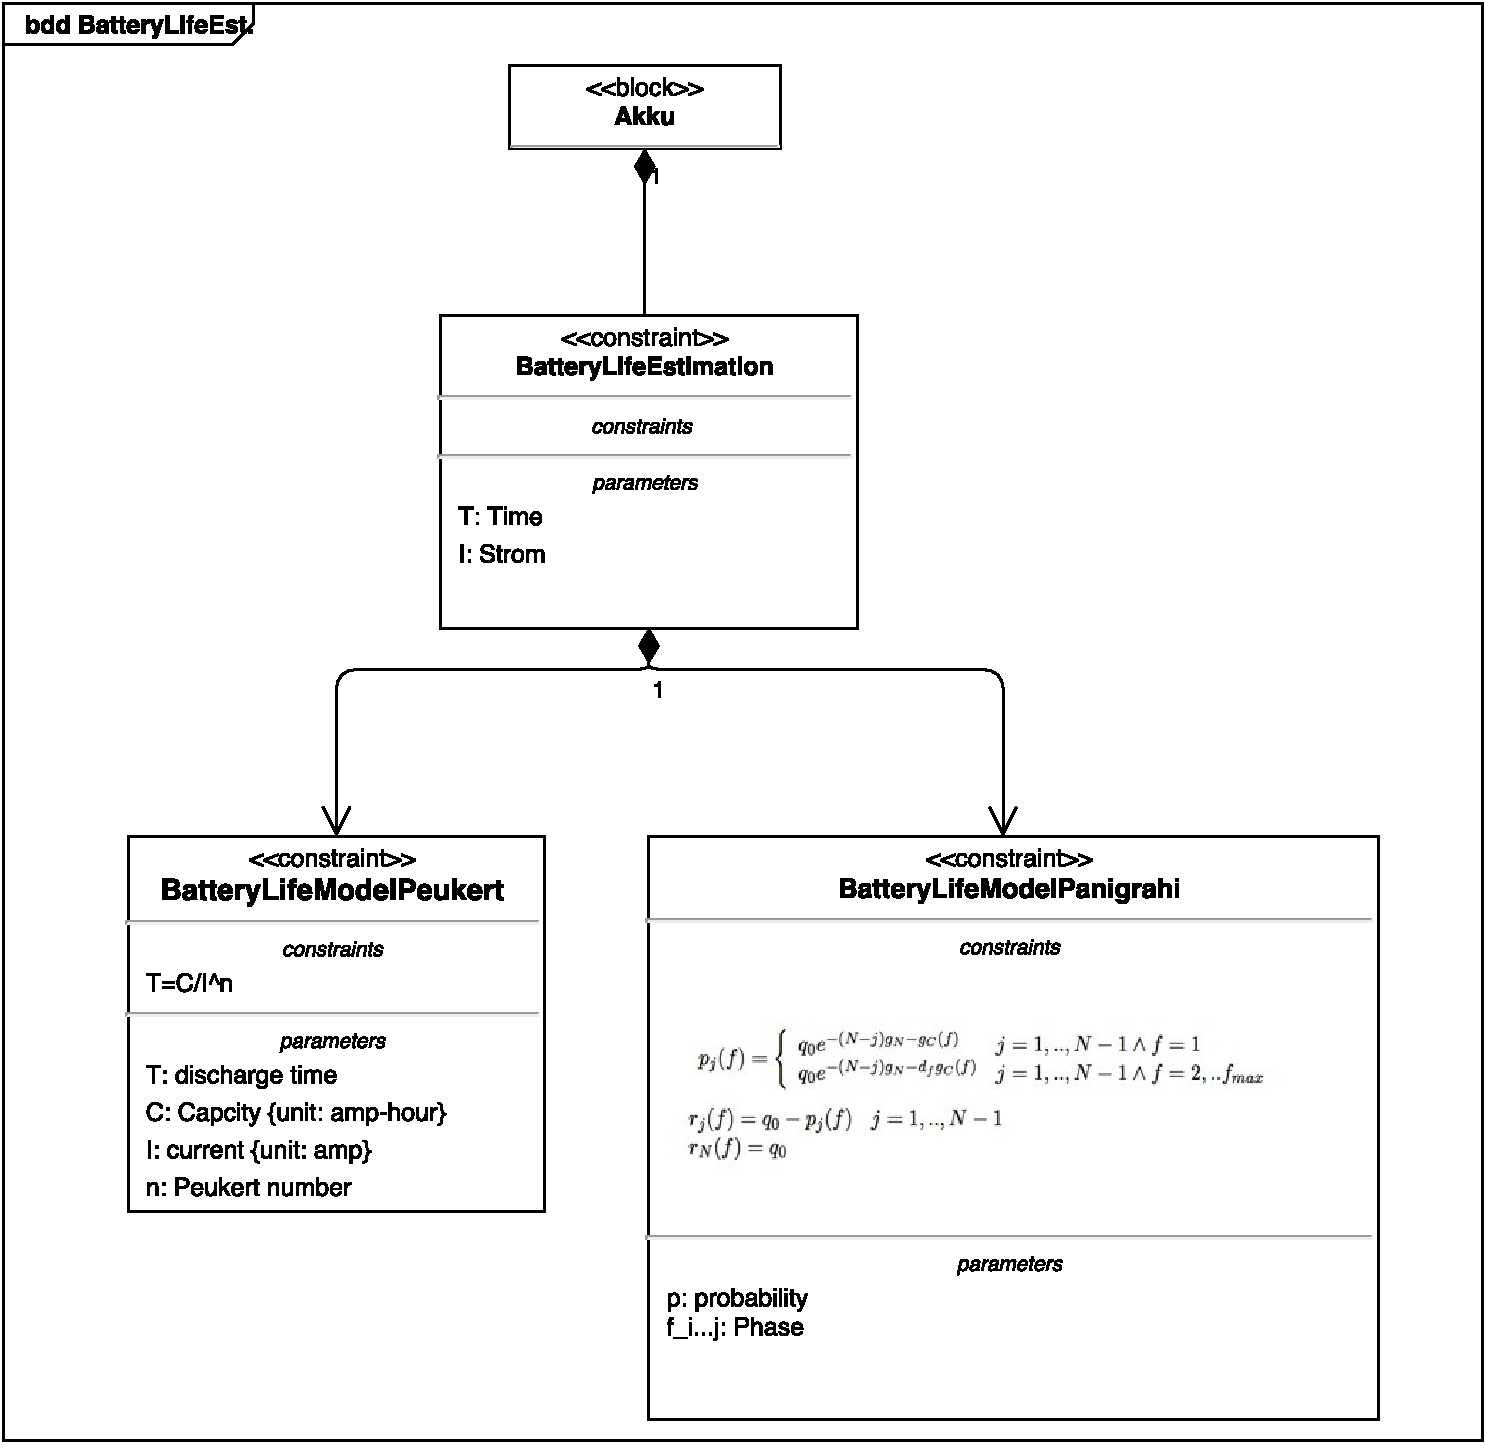
\includegraphics[width=10cm]{img/batterybdd}
\caption{Block Definition Diagram mit den einzelnen Constraint Blöcken}\label{fig:blockBattery}
\end{figure}

Die Verbindungen der einzelnen Systemeigenschaften mit den Constraint-Parameter ist in 
Abbildung \ref{parBattery} dargestellt.
In diesem Diagramm kann man die Beziehungen zwischen den Parametern der einzelnen Constraints und den Systemeigenschaften, hier sind es die Sensoren sehen.

\begin{figure}[H]
\centering\
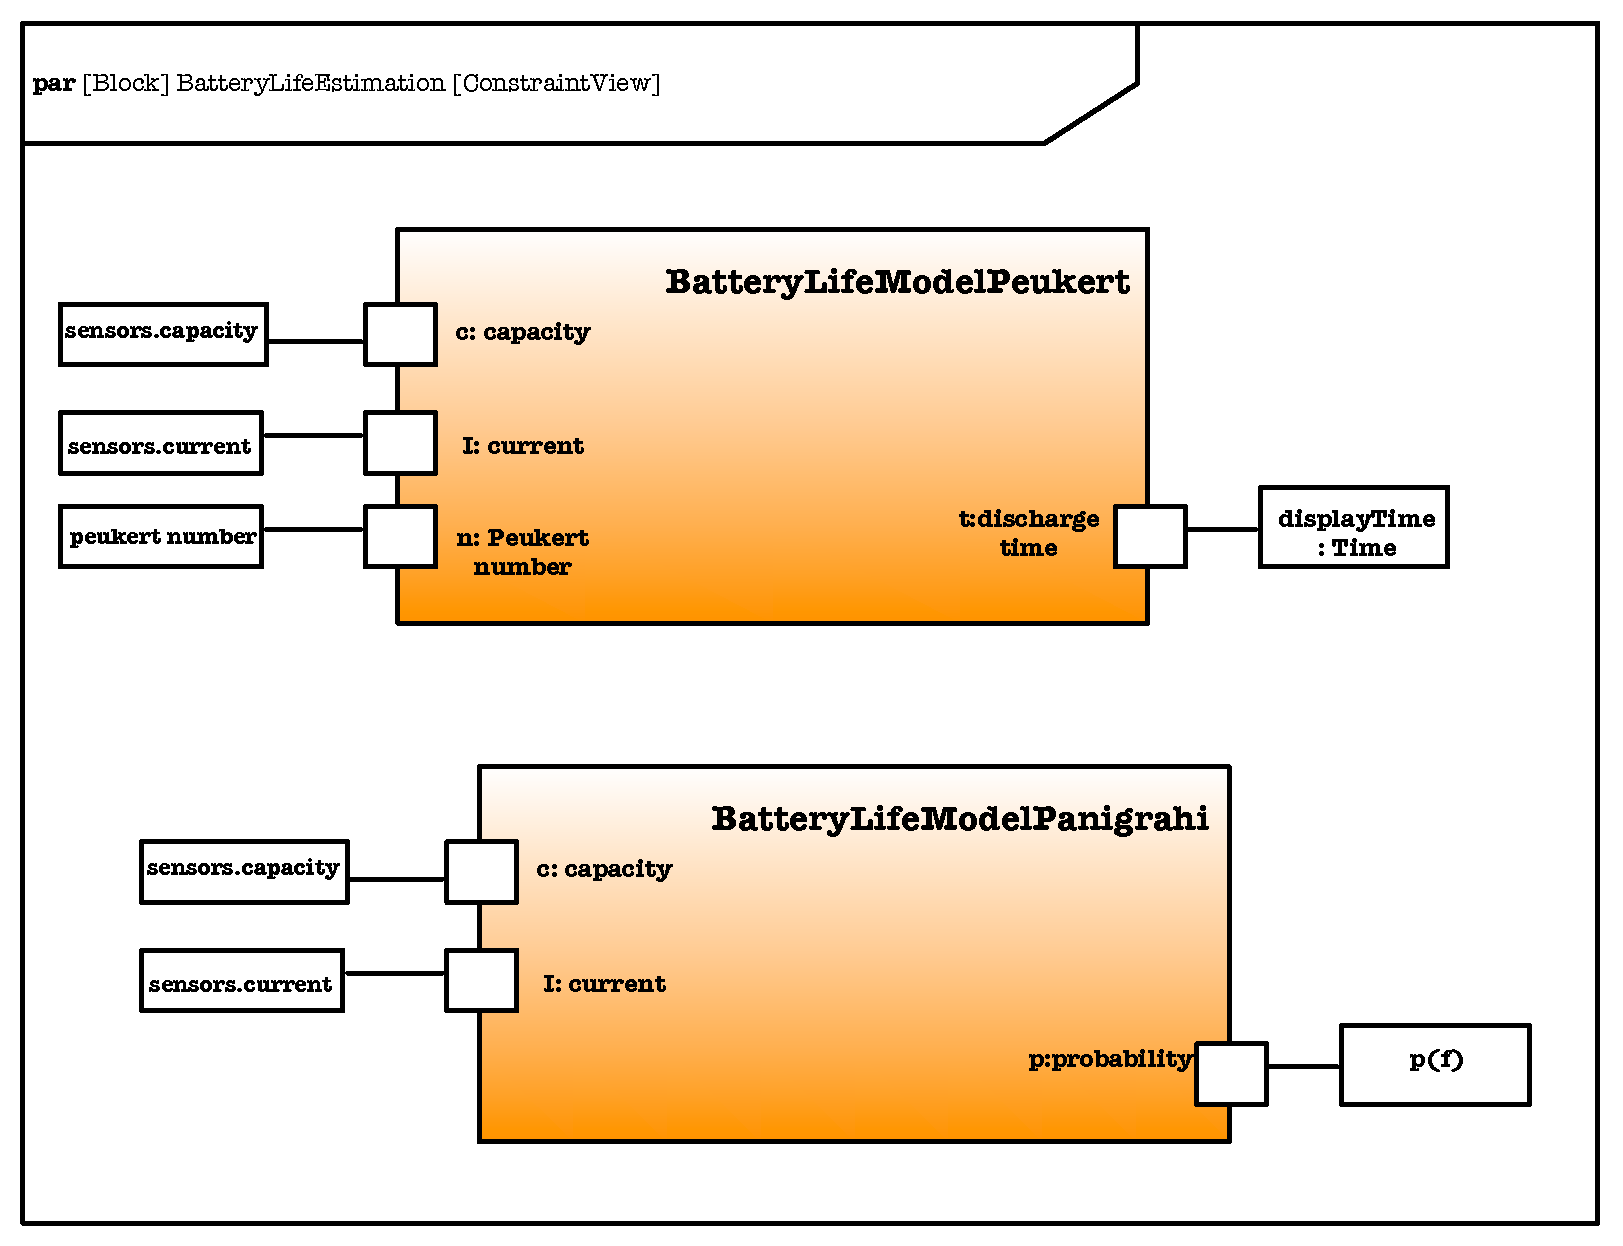
\includegraphics[width=10cm]{img/batteryParametric}
\caption{Parametric Diagram für die Conditions Akkulaufzeit}\label{fig:parBattery}
\end{figure}


\section{Activity Diagram}
In der abschließenden Phase des Projekts, wurden die für uns am häufigsten auftretenden Interaktionen zwischen Benutzer und \textit{SmartWatch} als Aktivität dargestellt. Diese sind unserer Ansicht nach, das \textit{Laden der Uhr}, das \textit{Starten von Apps} und die \textit{Telefon -und Mitteilungsfunktionalität}.\\
\begin{figure}[h]
\centering\
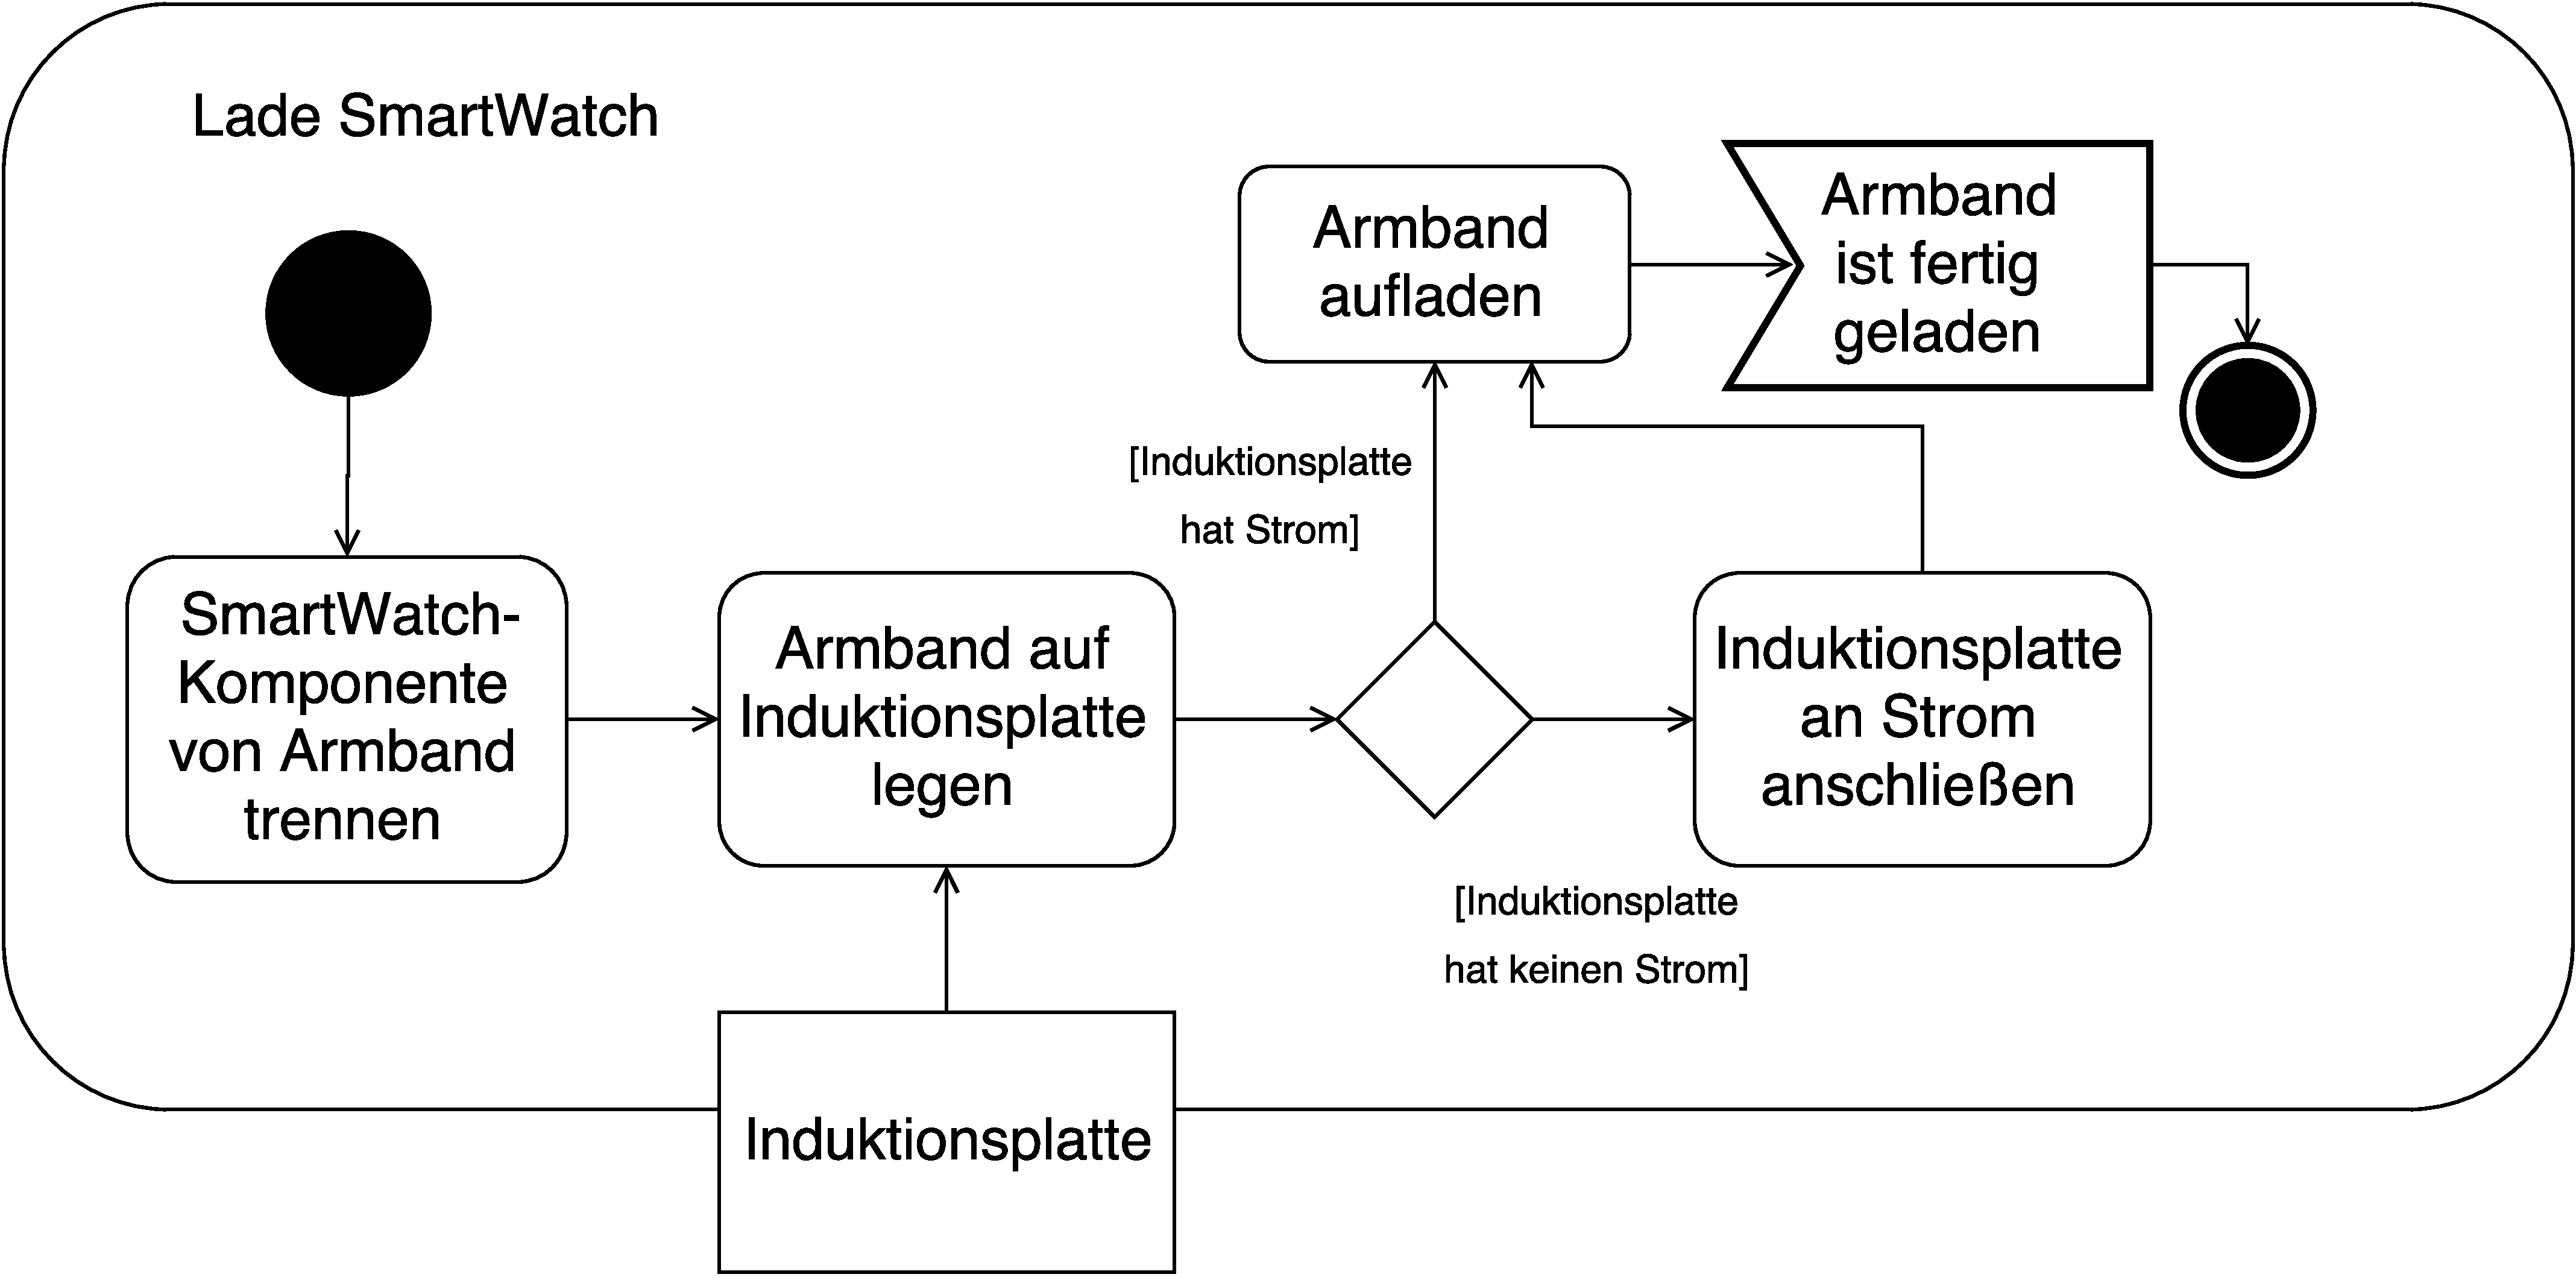
\includegraphics[width=\textwidth]{img/activityLaden}
\caption{Laden des SmartWatch-Armbandes über die mitgelieferte Induktionsplatte.}\label{fig:activityLaden}
\end{figure}
Zunächst betrachten wir den \textit{Ladevorgang} der \textit{SmartWatch} in Abbildung \ref{fig:activityLaden}.
Um die \textit{SmartWatch} laden zu können, muss das \textit{Uhren-Modul} zunächst vom \textit{Armband} getrennt werden. Geladen wird die Uhr per \textit{Induktion} über eine mitgelieferte \textit{Induktionsplatte}. Das \textit{Armband} wird nur geladen, sofern die \textit{Induktionsplatte} am \textit{Stromnetz} angeschlossen wird.  \\
\begin{figure}[h]
\centering\
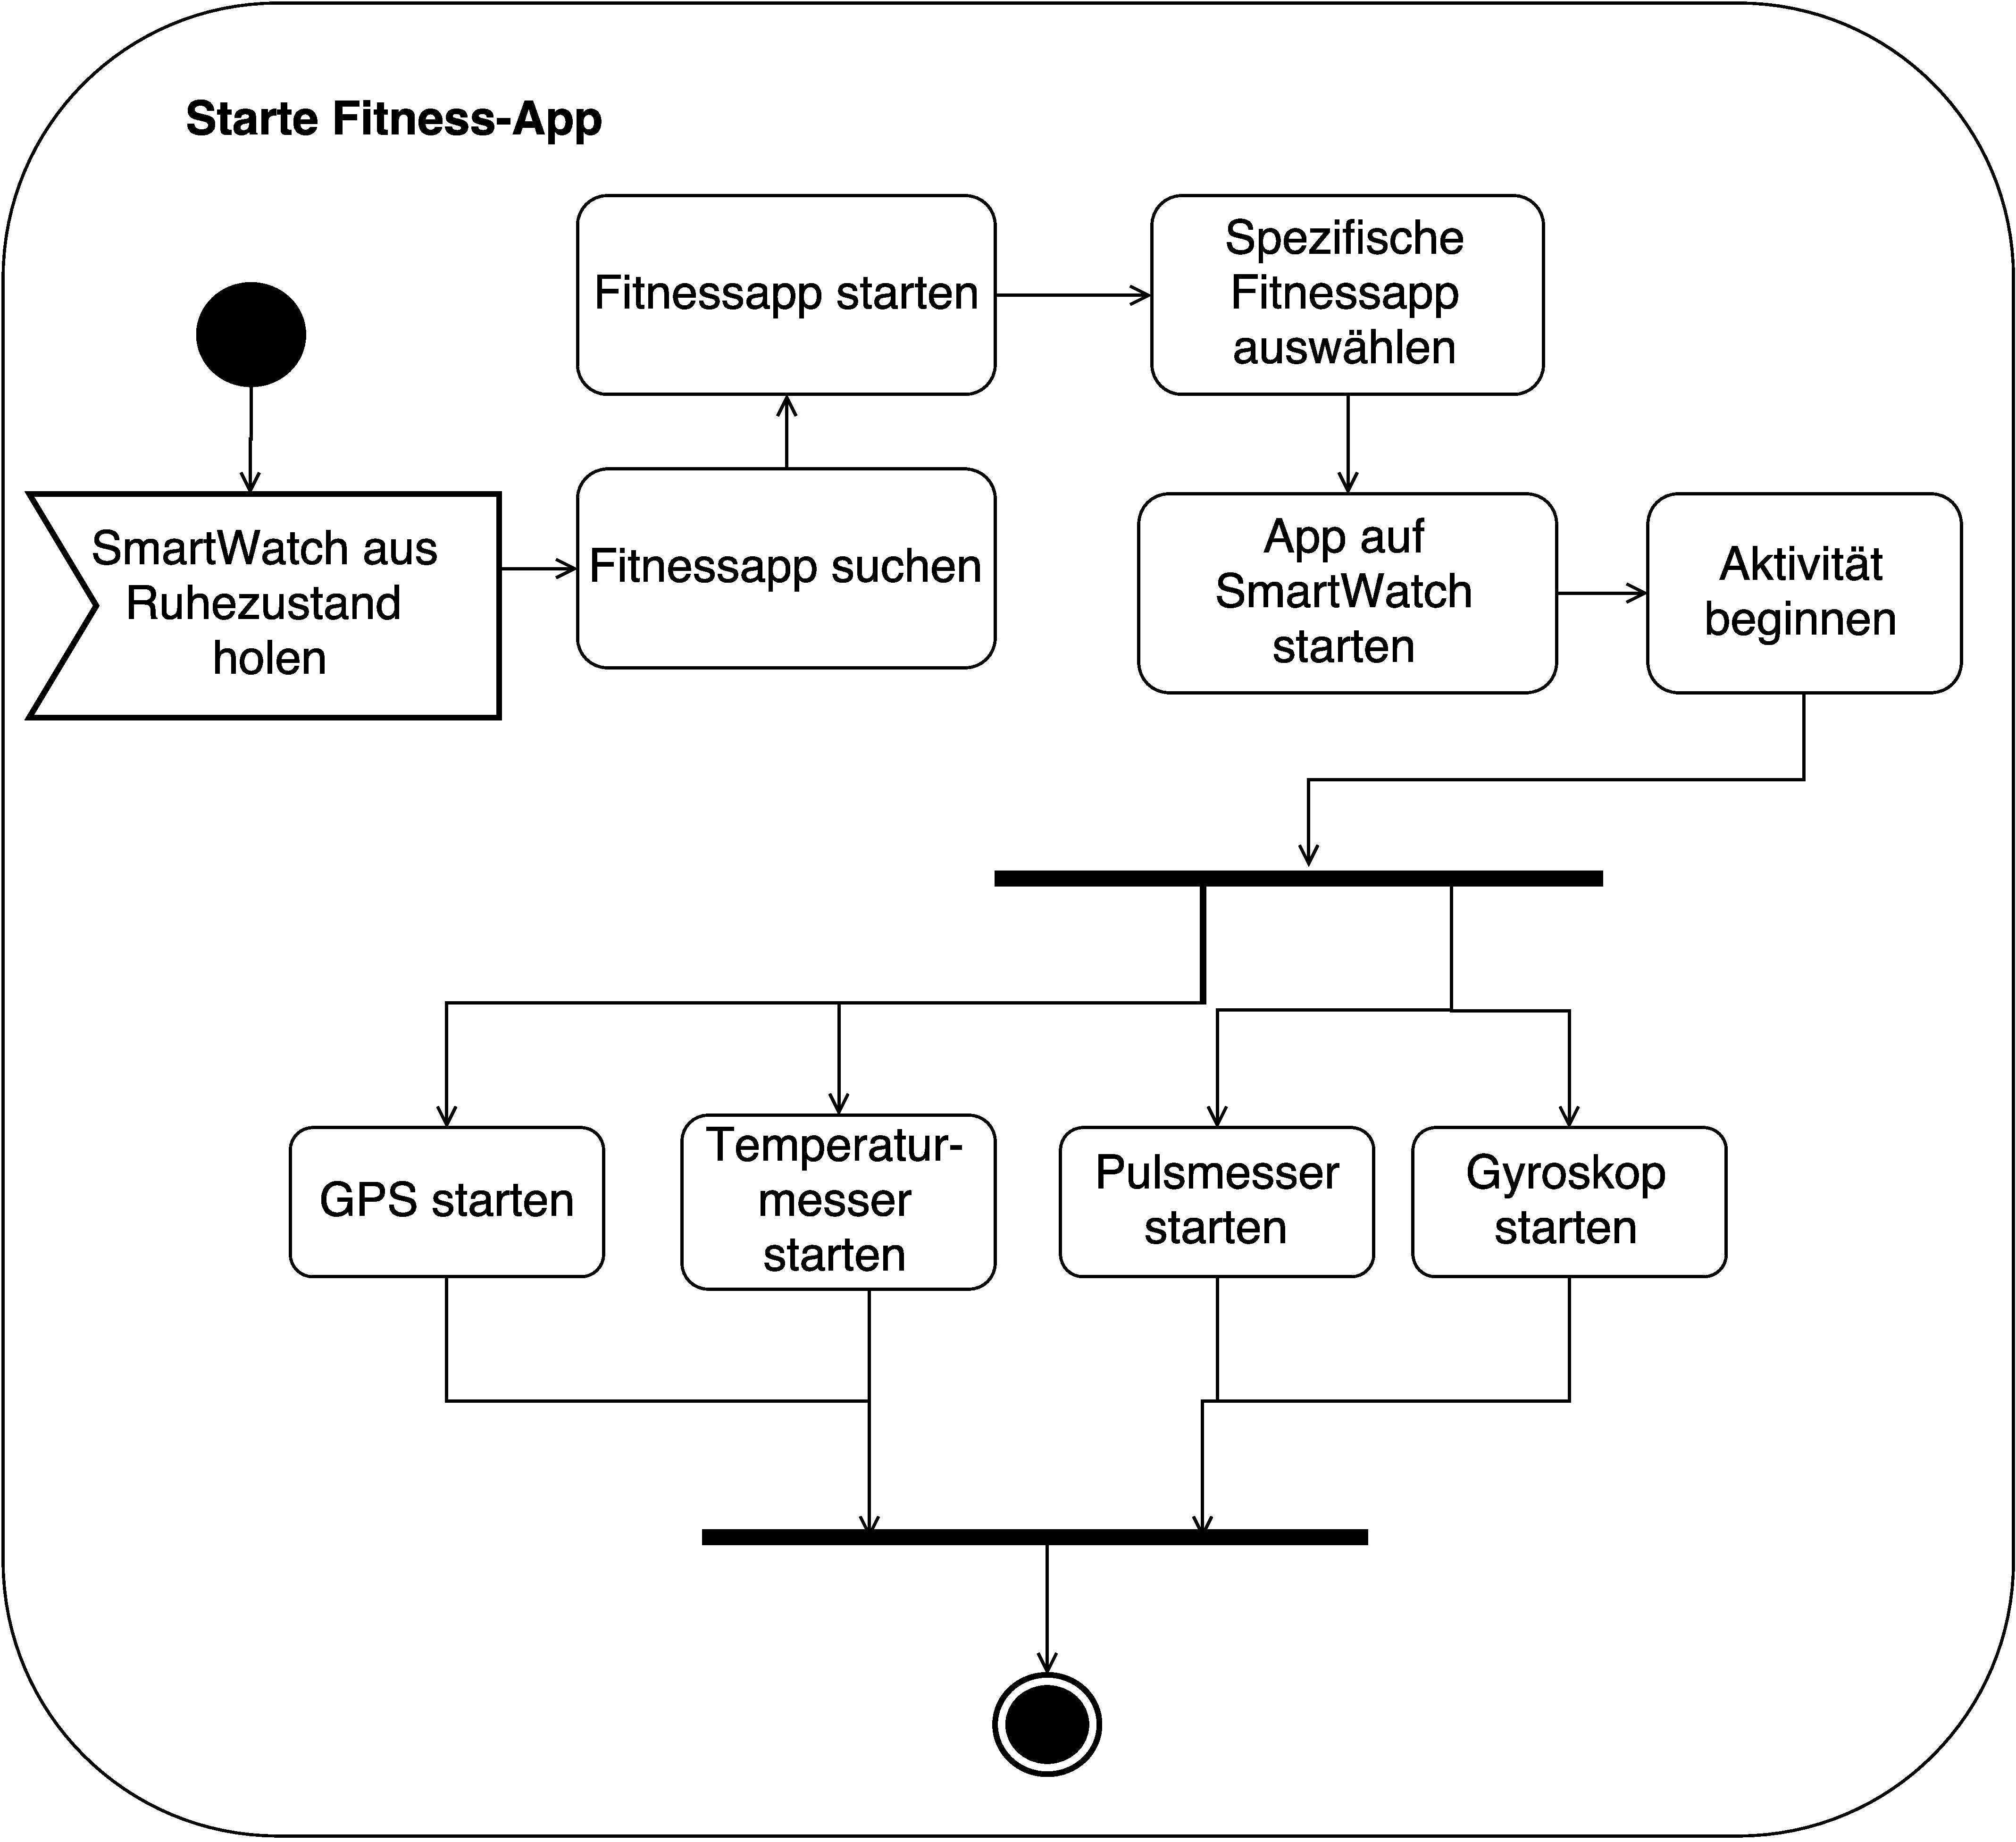
\includegraphics[width=\textwidth]{img/activityFitness}
\caption{Starten einer Fitnessapp durch den Benutzer.}\label{fig:activityFitness}
\end{figure}
Da die \textit{SmartWatch} über \textit{native Fitnessapplikationen} verfügt, werden diese anders als die \textit{normalen SmartPhone-Applikationen} gestartet (Abb. \ref{fig:activityFitness}).
Für das Starten einer \textit{Fitnessapplikation} wird die \textit{SmartWatch} zunächst aus dem Ruhezustand geholt. Sobald die \textit{SmartWatch} betriebsbereit ist, kann man über das \textit{Appmenü} die \textit{Fitnessapp} suchen und aktivieren. Daraufhin erscheint eine Liste mit verschiedenen \textit{spezifischen Aktivitäten}, wie z.B. \textit{Laufen} oder \textit{Fahrradfahren}. Sobald die \textit{Aktivität} ausgewählt und gestartet wurde, werden auf der \textit{SmartWatch} das \textit{GPS}, der \textit{Temperatursensor}, der \textit{Pulsmesser}, und das \textit{Gyroskop} aktiviert. \\
\begin{figure}[h]
\centering\
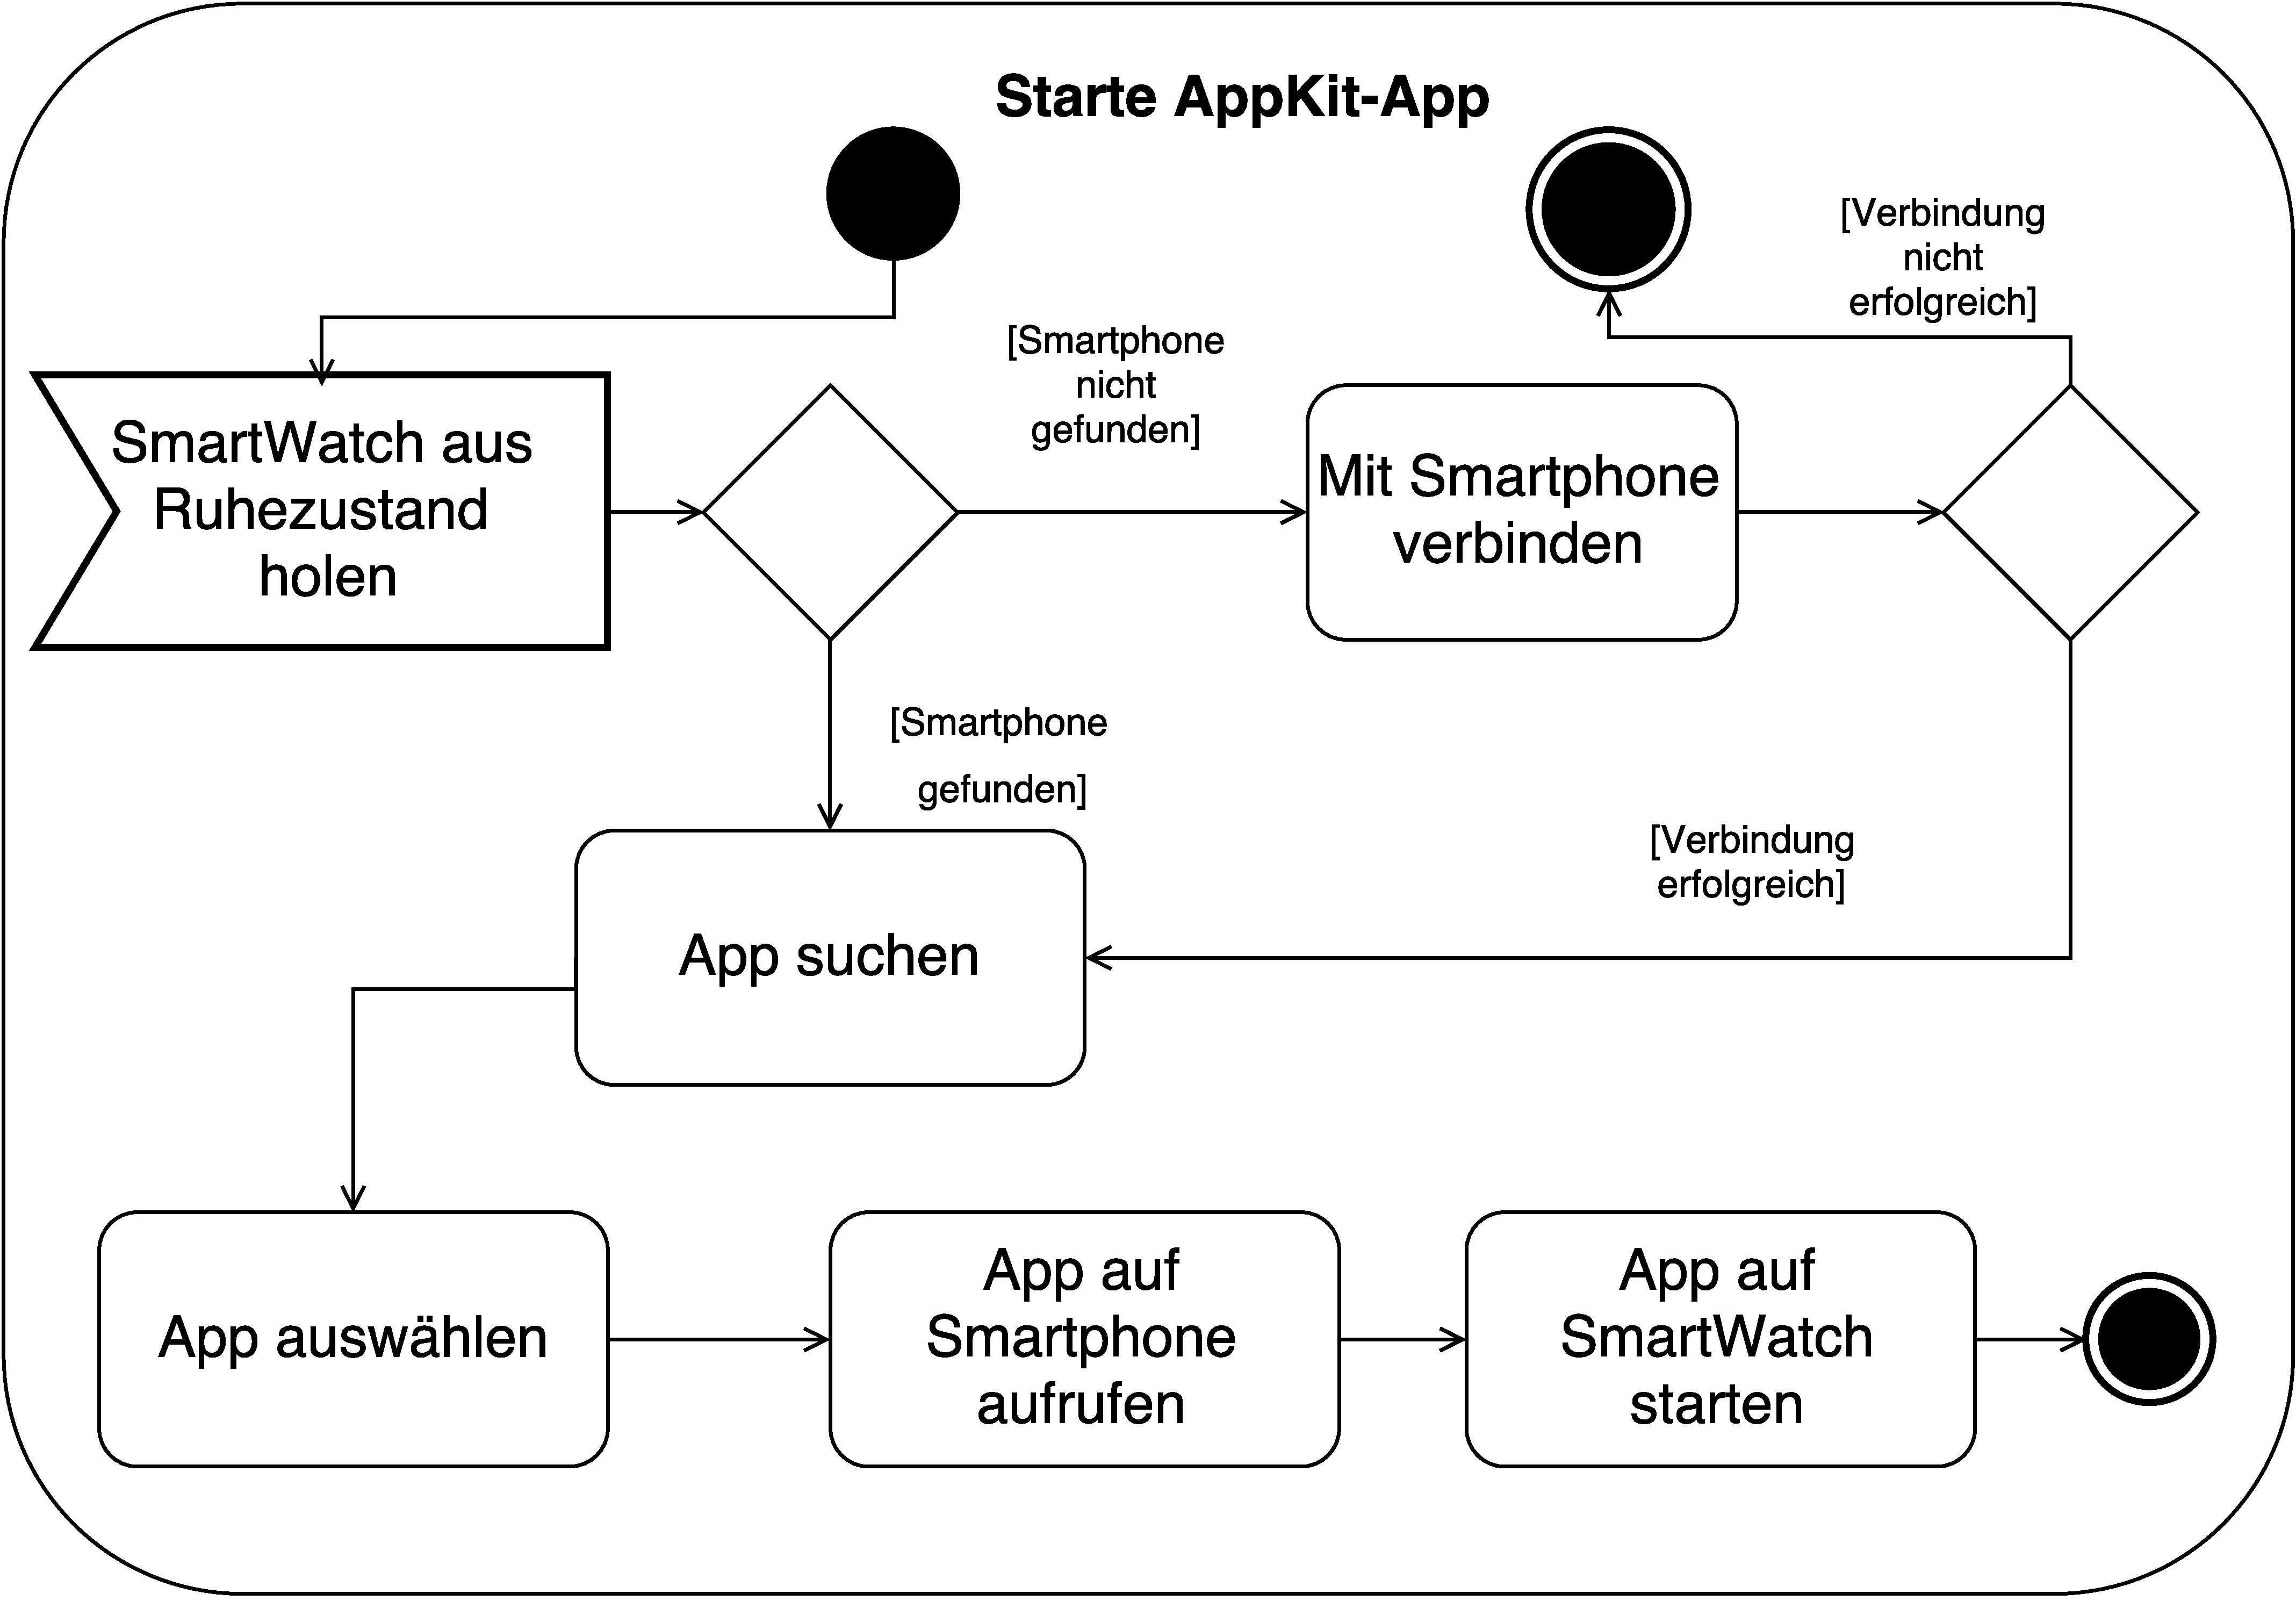
\includegraphics[width=\textwidth]{img/activityAppKit}
\caption{Starten einer AppKit-Applikation durch den Benutzer.}\label{fig:activityAppKit}
\end{figure}
Da die \textit{Fitnessfunktionalität} keine Verbindung zum \textit{SmartPhone} erfordert, unterscheidet sich das Starten einer normalen Applikation (Abb. \ref{fig:activityAppKit}). Auch hierfür muss die \textit{SmartWatch} zunächst aus ihrem \textit{Ruhezustand} geholt werden. Zunächst überprüft die \textit{SmartWatch} über das \textit{Appmenü}, ob überhaupt eine Verbindung zum \textit{SmartPhone} besteht, bevor auf dessen \textit{Applikationen} zugegriffen werden kann. Nur bei einer erfolgreichen Verbindung werden die \textit{Programme} des \textit{Telefons} auf der \textit{SmartWatch} angezeigt. Nachdem eine \textit{Applikation} ausgewählt wurde, wird diese zunächst auf dem \textit{SmartPhone} ausgeführt. Über die \textit{Bluetooth-Schnittstelle} lässt sich nun das \textit{Programm} über das \textit{SmartWatch-Interface} steuern.\\
\begin{figure}[h]
\centering\
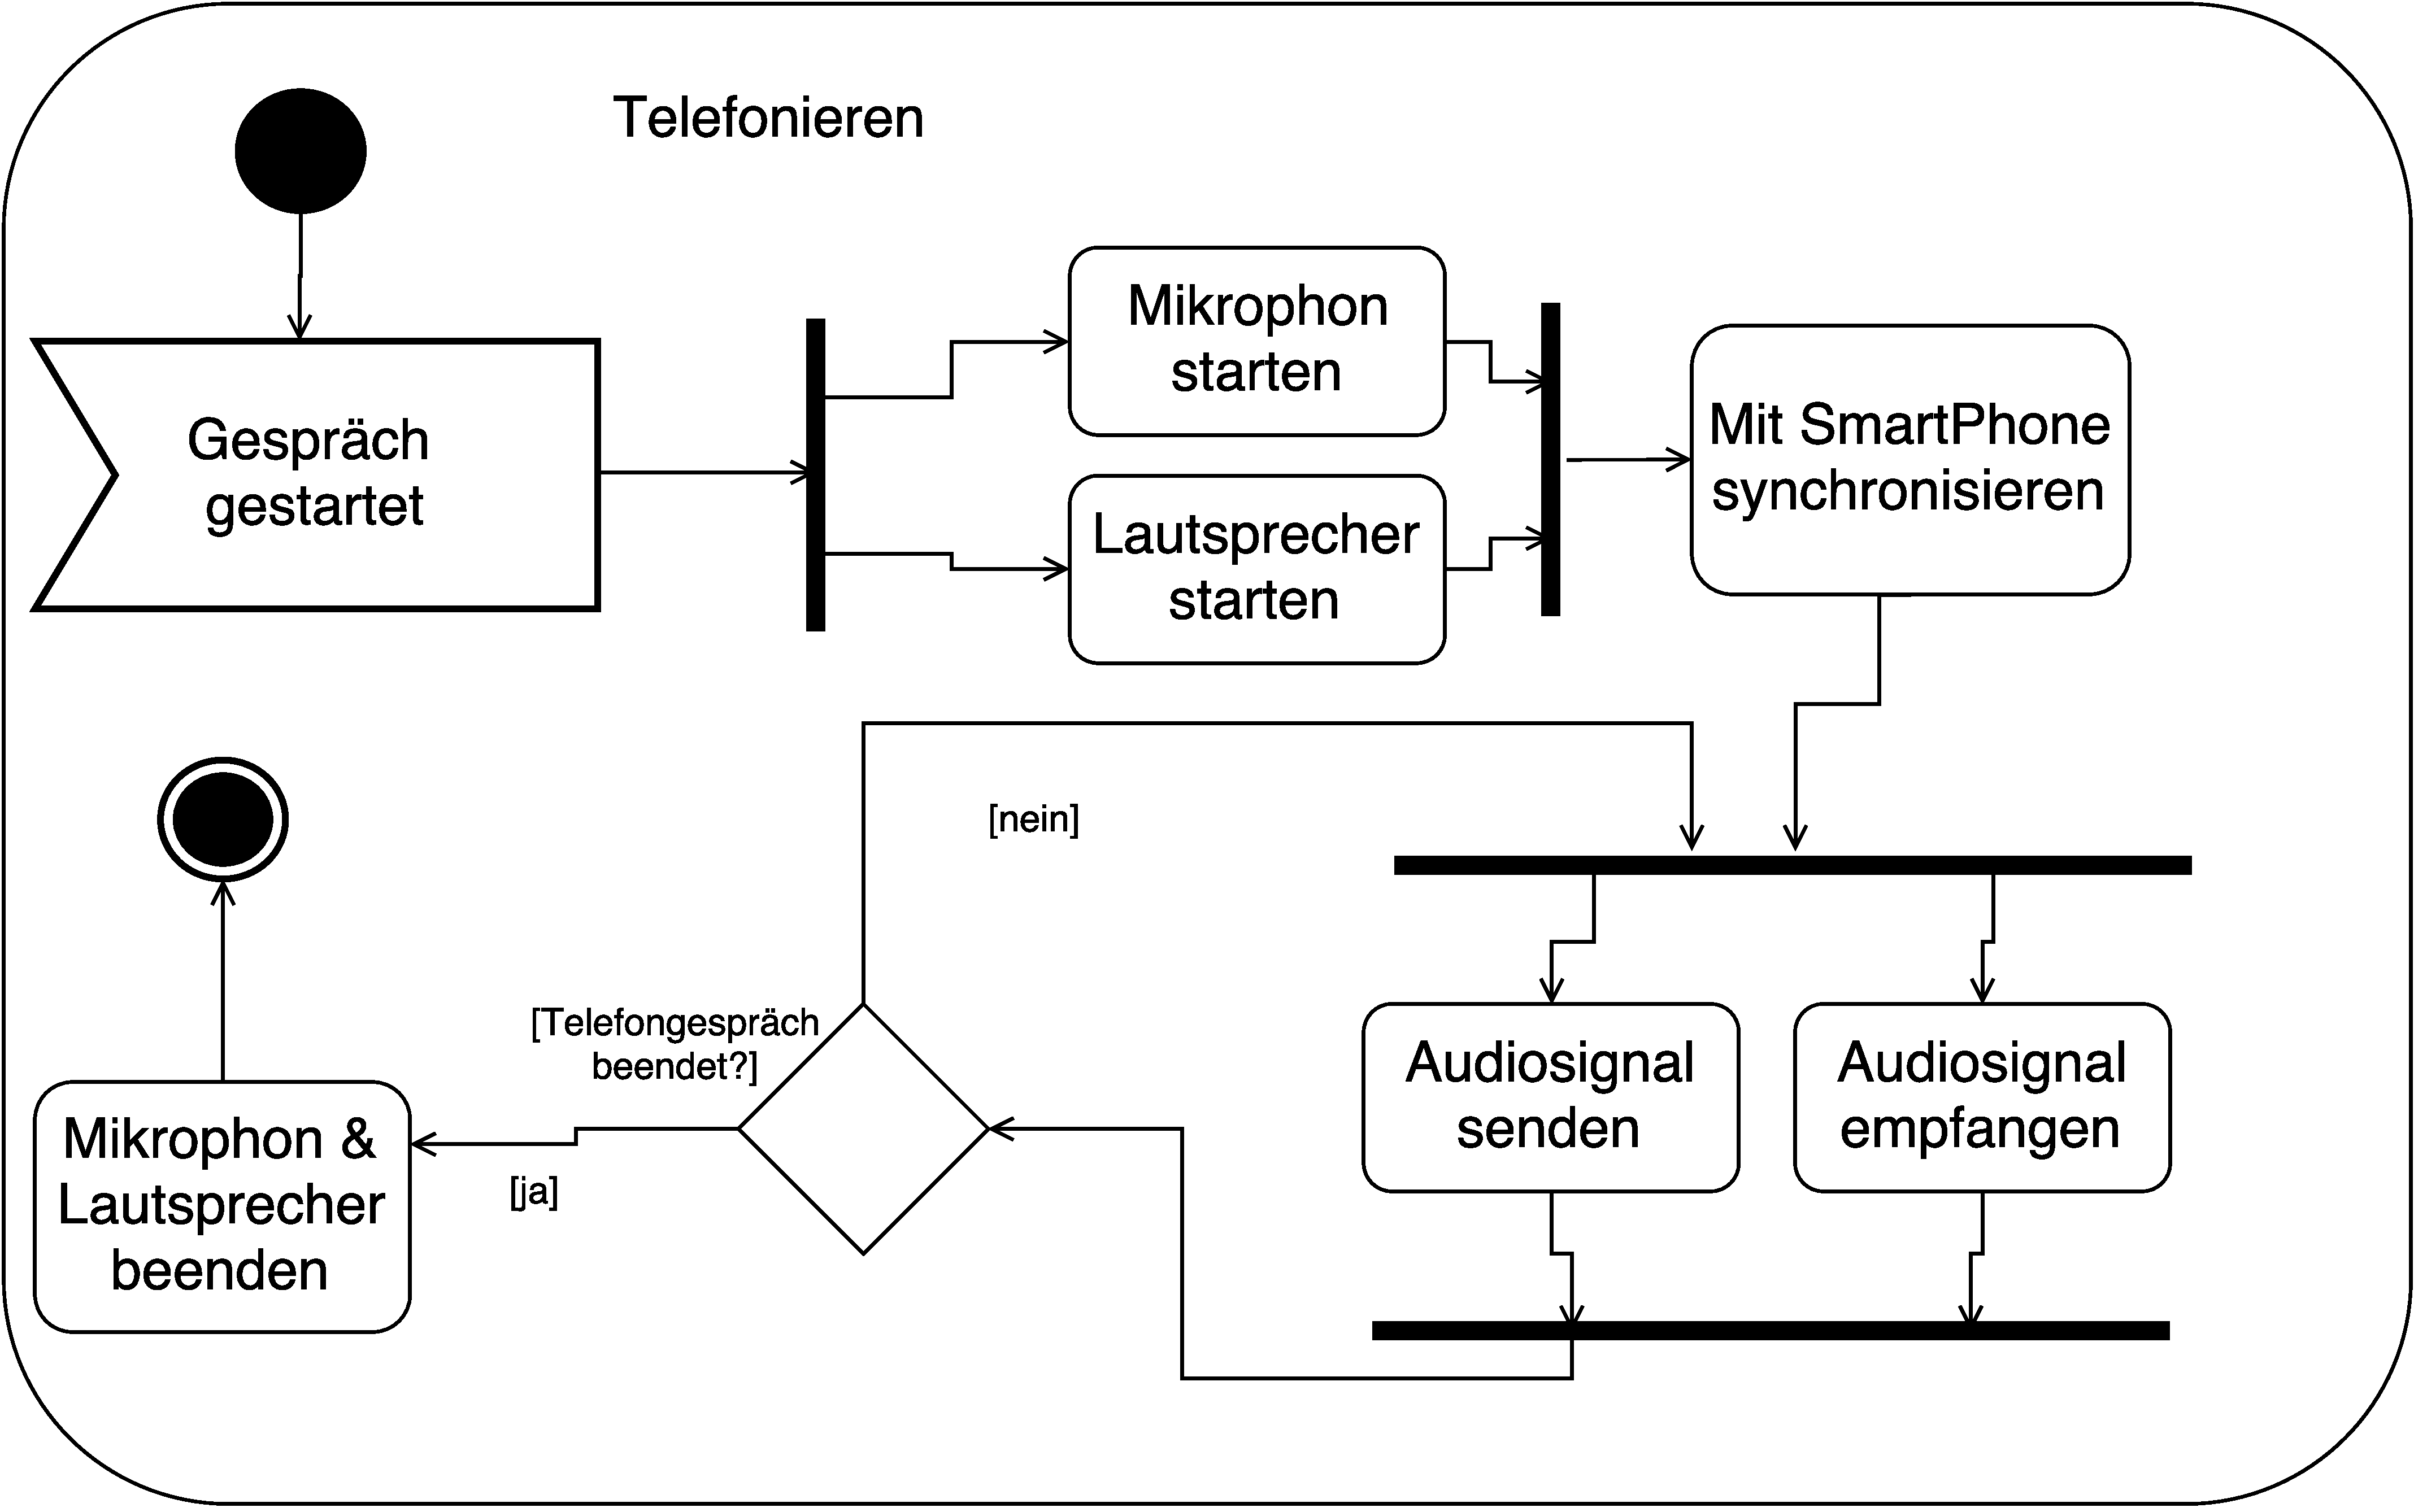
\includegraphics[width=\textwidth]{img/activityTelefonieren}
\caption{Verhalten der SmartWatch bei einem Telefonat.}\label{fig:activityTelefonieren}
\end{figure}
Als Nächstes wird die \textit{Telefonieren} Aktivität betrachtet (Abb. \ref{fig:activityTelefonieren}). Dieses Diagramm beschreibt das Verhalten der \textit{Uhr} bei einem bereits \textit{angenommenen Gespräch}. Hier wird davon ausgegangen, dass bereits eine bestehende Verbindung zwischen \textit{SmartWatch} und \textit{SmartPhone} besteht. Sobald das \textit{Gespräch} begonnen wurde, werden \textbf{parallel} das \textit{Mikrophon} und der \textit{Lautsprecher} der \textit{Uhr} gestartet und mit dem \textit{SmartPhone} synchronisiert. Das bedeutet, dass jeder Spracheingang und Audioausgang, der sonst über das \textit{SmartPhone} stattfinden würde, stattdessen über die \textit{SmartWatch} abgewickelt wird. So können über die \textit{Uhr} \textbf{parallel} \textit{Audiosignale gesendet} und \textit{empfangen} werden. Dies geschieht so lange, bis das \textit{Telefonat} beendet wird. Anschließend werden sowohl \textit{Mikrophon} als auch \textit{Lautsprecher} beendet.\\
\begin{figure}[h]
\centering\
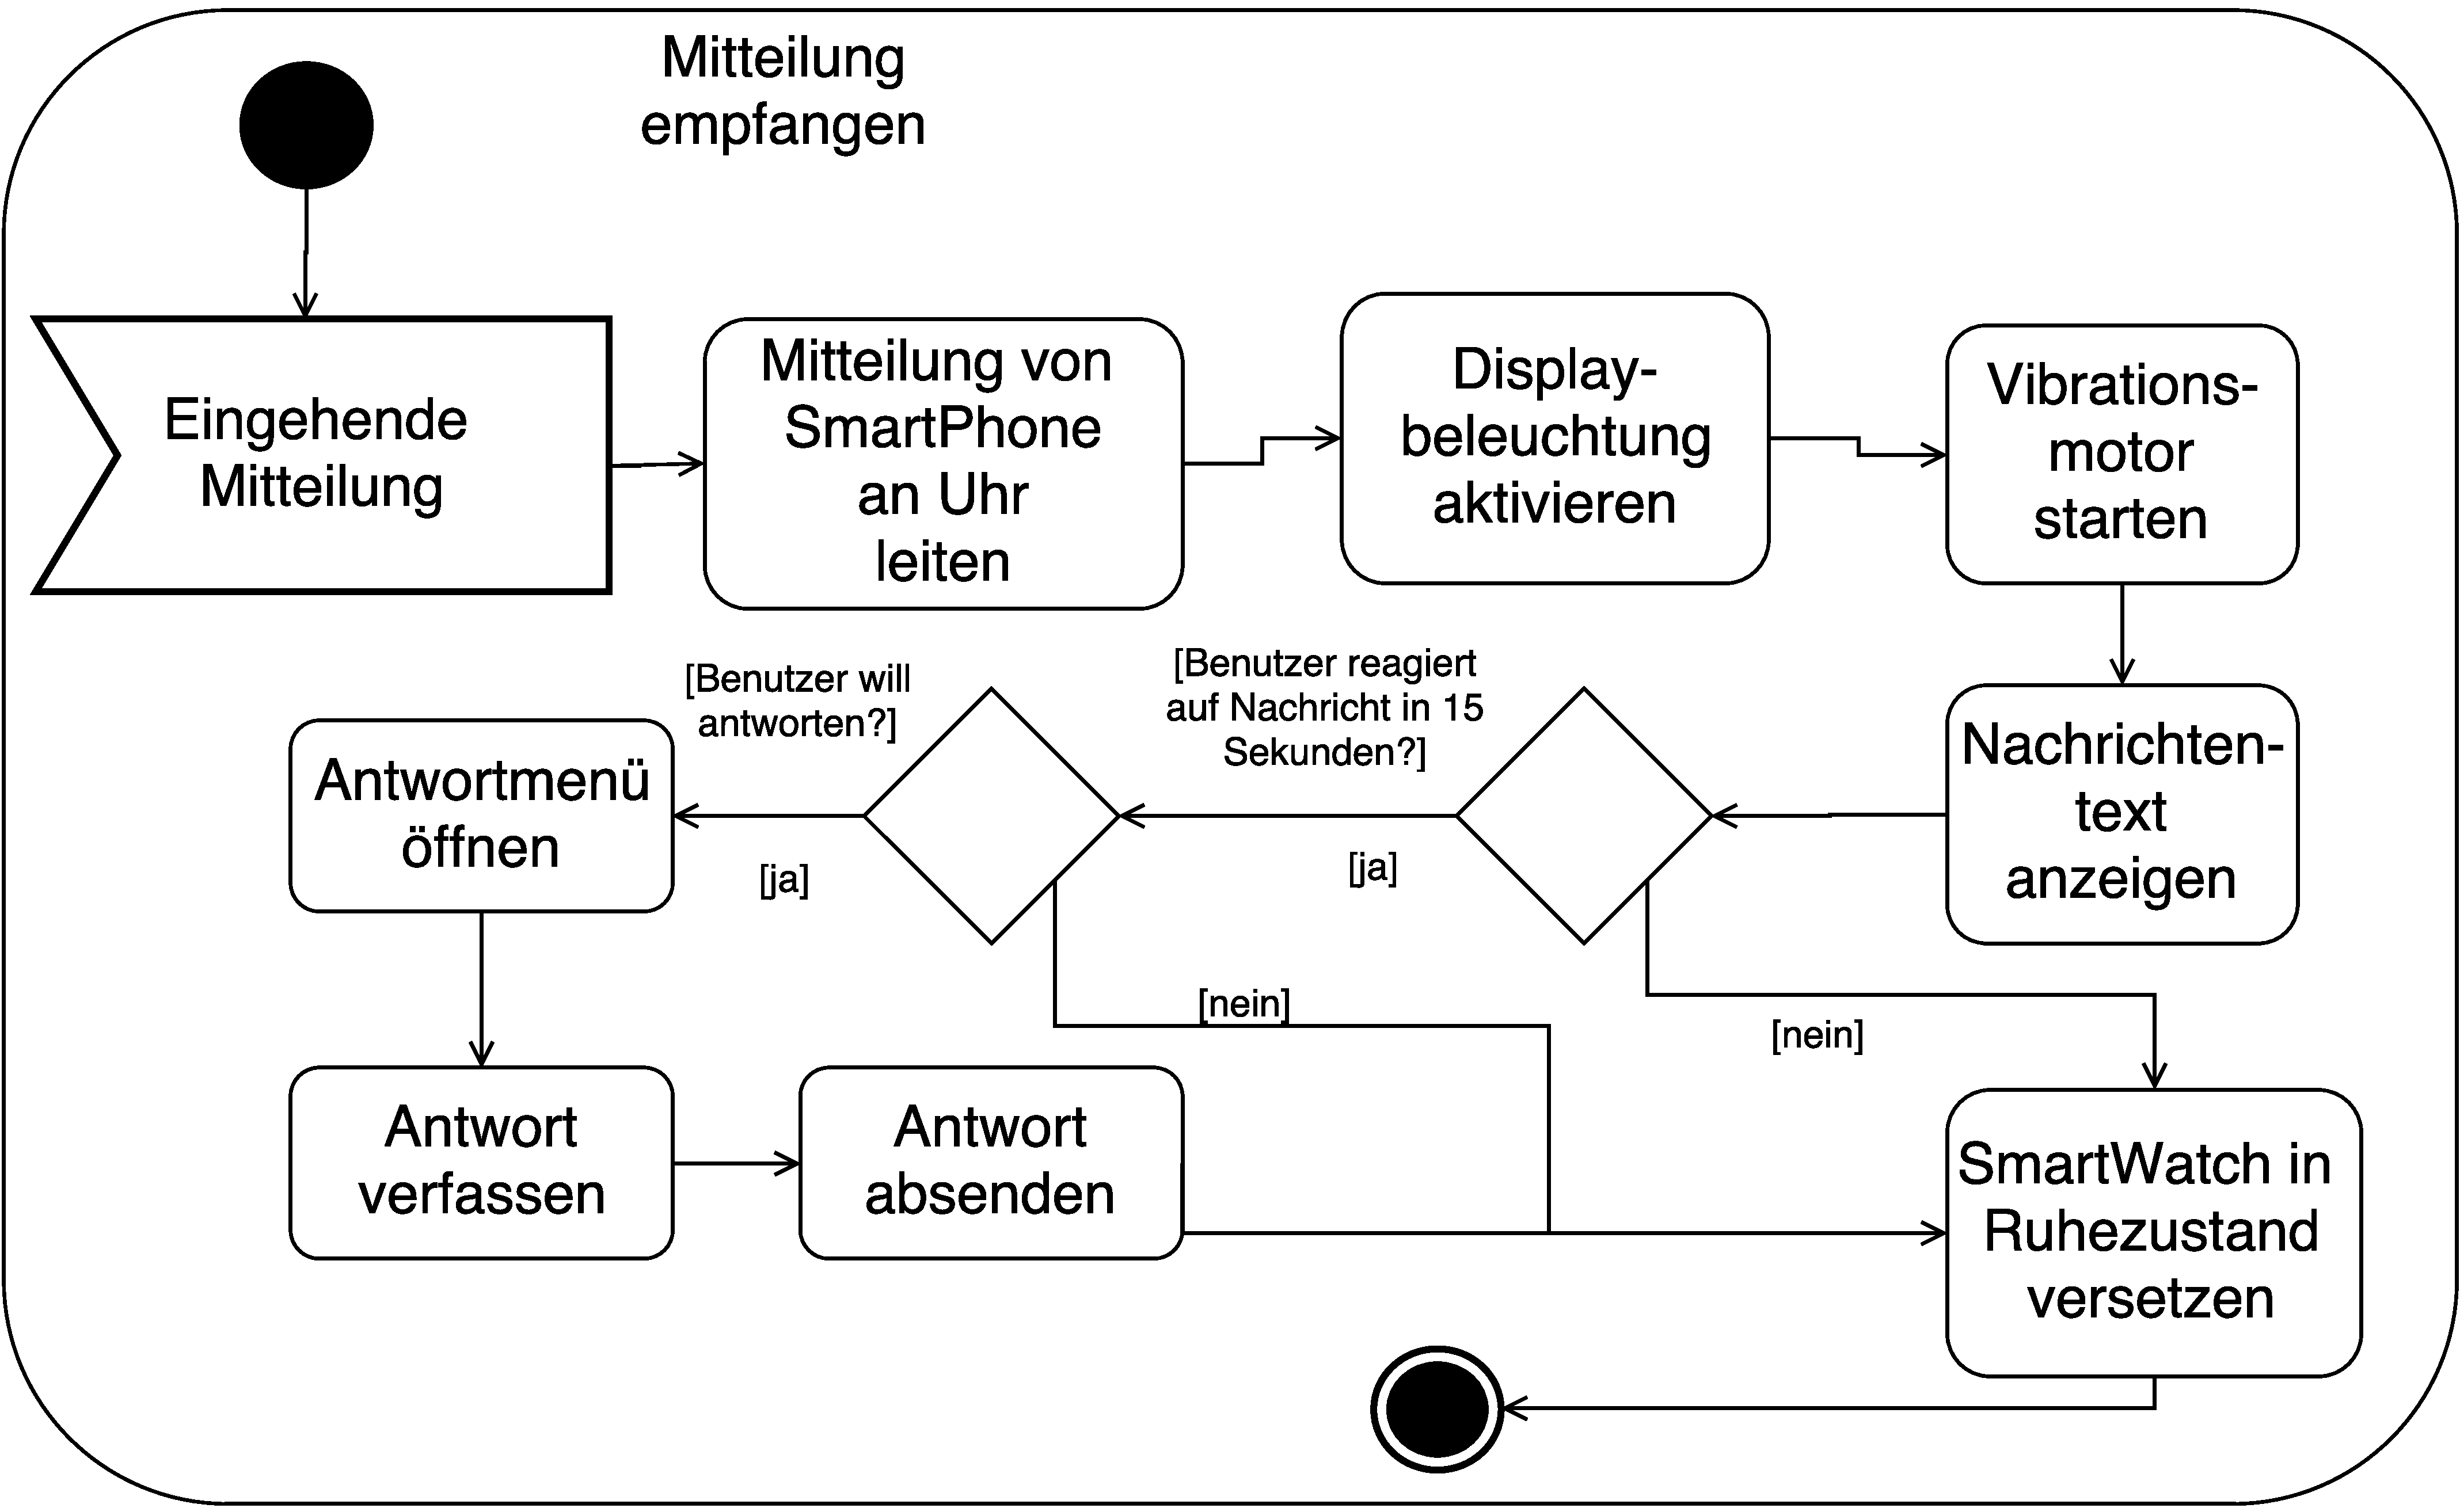
\includegraphics[width=\textwidth]{img/activityMitteilung}
\caption{Verhalten der SmartWatch bei einer eingehenden Mitteilung.}\label{fig:activityMitteilung}
\end{figure}
Zum Schluss wird betrachtet, was passiert, wenn auf dem \textit{Mobiltelefon} eine \textit{Mitteilung} eingeht (Abb. \ref{fig:activityMitteilung}). Die \textit{empfangene Nachricht} wird, nachdem sie auf dem \textit{SmartPhone} verarbeitet wurde, an die \textit{SmartWatch} weitergeleitet. Sobald die \textit{Uhr} die Nachricht empfangen hat, aktiviert sich die \textit{Displaybeleuchtung} und der \textit{Vibrationsmotor} beginnt sich zu drehen. Anschließend wird der \textit{Nachrichtentext} auf der Uhr ausgegeben. Das Verhalten hierbei kann sich aufgrund verschiedener Einstellungen von Ton und Vibration unterscheiden. Falls der \textit{Benutzer} nach \textbf{15 Sekunden} nicht auf die Nachricht reagiert, versetzt sich die \textit{SmartWatch} wieder in den \textit{Ruhezustand}. Sollte rechtzeitig auf die Nachricht reagiert werden, hat der \textit{Benutzer} die Möglichkeit zu antworten und das \textit{Antwortmenü} zu öffnen. Sobald der \textit{Benutzer} die Mitteilung verfasst hat, wird diese über das \textit{SmartPhone} abgesendet. Daraufhin beendet sich das \textit{Antwortmenü} und die \textit{SmartWatch} geht zurück in den \textit{Ruhezustand}.

\section{Sequence Diagram}

Das folgende Sequenzdiagramm zeigt das Szenario einer erhaltenen Mitteilung. Zu Beginn erhält die Smartphone die Nachricht ("message"). Die erhaltene Nachricht leitet er weiter an Smartwatch mit dem Operator sendMessage(). Danach wird die Nachricht am Display angezeigt, die Smartwatch schickt dem Display eine Nachricht mit showMessage() und zur selben Zeit kann eine Benachrichtigung stattfinden. Dabei gibt es vier Möglichkeiten einer Benachrichtigung.
1.: Die Bedingung ist, dass Vibration und Sound an ist. Die Smartwatch vibriert und anschließend kommt auch der Benachrichtigungston.
2.: Die Bedingung ist, dass die Vibration an ist und der Sound aus ist. Die Smartwatch vibriert, allerdings kommt kein Benachrichtigungston.
3.: Die Bedingung ist, dass die Vibration aus ist und der Sound an ist. Die Smartwatch vibriert nicht, stattdessen kommt ein Benachrichtigungston.
4.: else. Vibration und Sound sind aus.

\begin{figure}[H]
\centering\
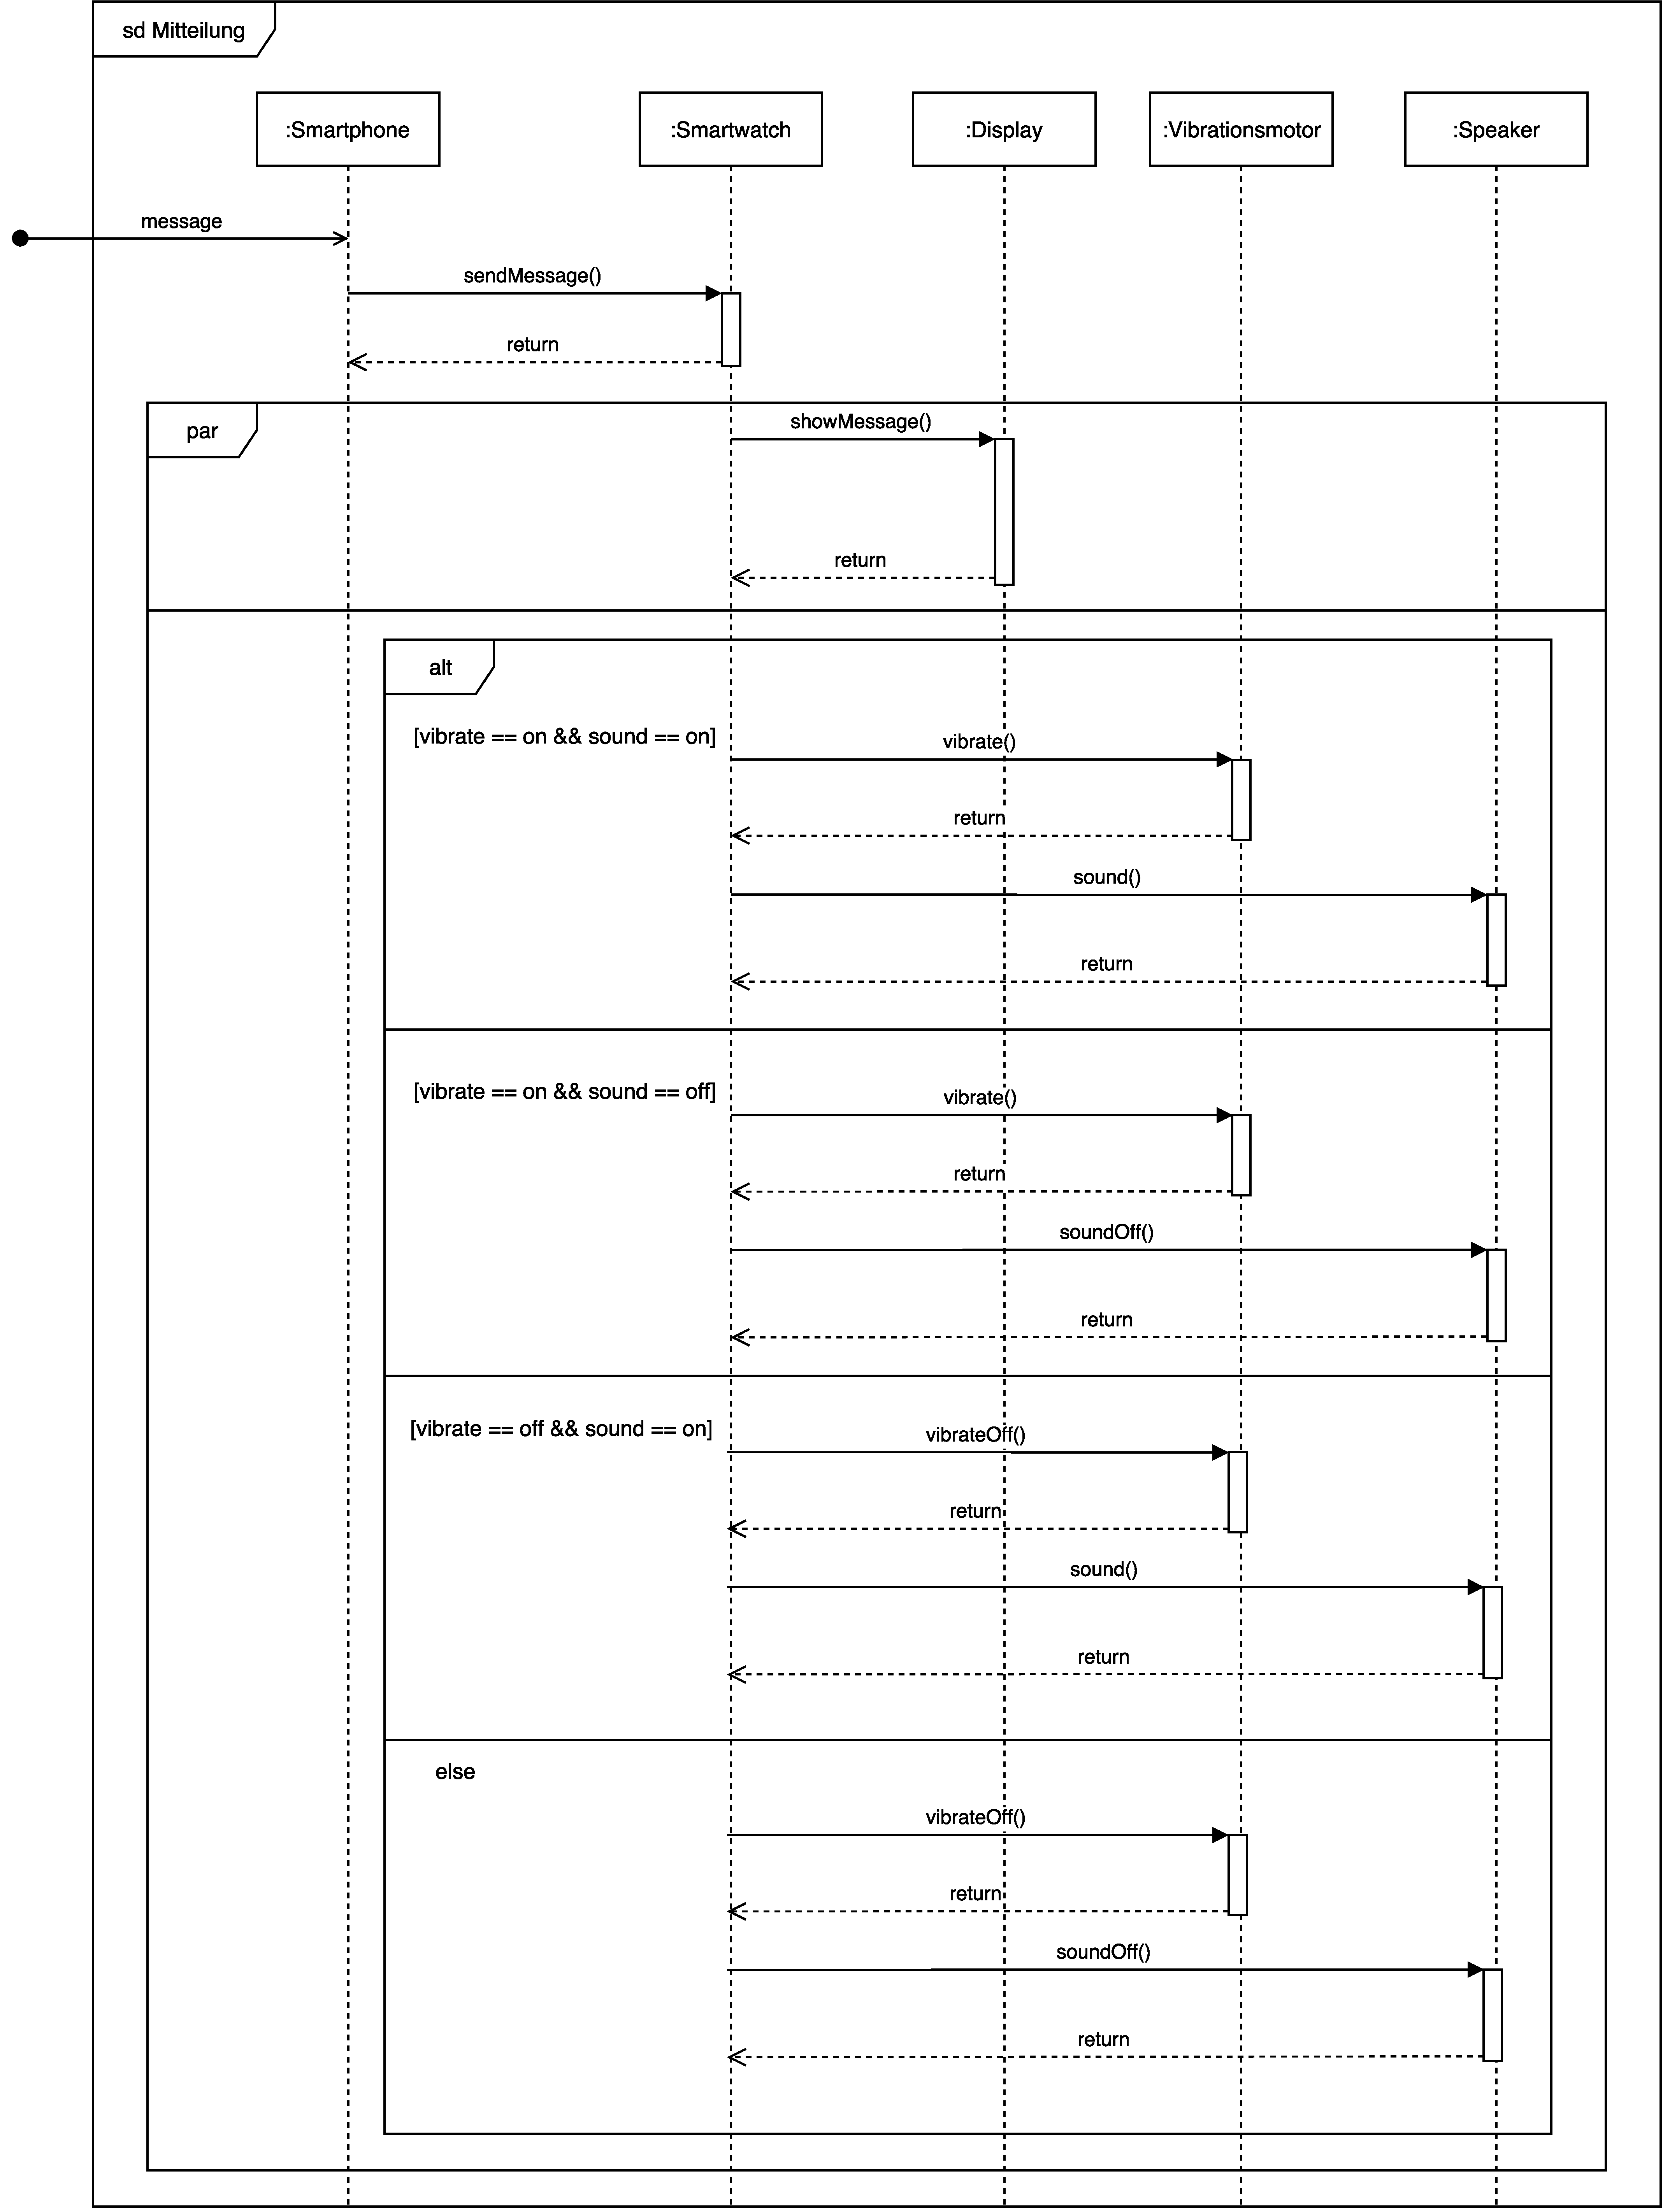
\includegraphics[width=\textwidth]{img/seqMessage}
\caption{Sequenzdiagramm zum erhalten einer Nachricht.}\label{fig:seqMessage}
\end{figure}
